\documentclass[11pt]{article}

% AMS Packages
\usepackage{amsmath} 
\usepackage{amssymb} 
\usepackage{amsthm}
% Page dimensions
\usepackage[margin=0.9in]{geometry}
% Images
\usepackage[pdftex]{graphicx} 
% Enumerate package
\usepackage{enumitem} 
\usepackage{array} 
% Fancify pages
\usepackage{fancyhdr} 
% Convert captions on figures to bold font
\usepackage[labelfont=bf,textfont=md]{caption}
% Time New Roman font
\usepackage{times}
% package to set line spacings
\usepackage{setspace} 
% SI Units in math type
\usepackage{siunitx}
\usepackage{textcomp} 
% Change sizes of sections
\usepackage{titlesec}
\titleformat{\section}{\normalfont\large\bfseries}{\thesection}{1em}{}
\titleformat{\subsection}{\normalfont\bfseries}{\thesubsection}{1em}{}
\titleformat{\subsubsection}{\normalfont\small\bfseries}{\thesubsubsection}{1em}{}
% Declare useful math operators
\DeclareMathOperator*{\argmin}{arg\,min}
\DeclareMathOperator*{\plim}{plim}
\DeclareMathOperator{\Tr}{Tr}
\usepackage{float}


\begin{document}
\section{UoI$_\text{Lasso}$ Stability Selection}
	Union of Intersections (UoI) enforces a strict intersection of supports over bootstraps in its traditional implementation. To be clear, suppose we have $B_1$ bootstraps in the selection module; then, a feature must be selected in all $B_1$ bootstraps (of $\lambda_i$) to be passed along in the proposed support for the regularization strength $\lambda_i$. We can relax this assumption by only requiring that a feature appear in some fraction $f_s$ of the bootstraps, i.e. it appears in $f_s B_1$ selection bootstraps where $0 < f_s \leq 1$. Choosing $f_s$ wisely can result in a reduction of false negatives since we are softening the requirements for a feature to be selected.
	
	We have a problem, though: we must choose $f_s$ wisely. In effect, it becomes another hyperparameter in the optimization procedure. One approach is to let the UoI algorithm choose $f_s$ in a similar fashion that it chooses the regularization strength $\lambda$. Traditional UoI would pass $N_{\lambda}$ supports to the estimation module, where $N_{\lambda}$ is the number of $\lambda$ values. We could instead pass $N_{\lambda} \times N_{f_s}$ supports to the estimation module, where we apply $N_{f_s}$ selection thresholds to each of the original $N_{\lambda}$ supports. This serves as the natural extension of UoI to the case of multiple hyperparameters.
	
	Stability selection would be particularly useful in the case of collinear features. Two highly collinear features might be selected in different supports in lieu of each other, diluting their appearance in the supports of the $B_1$ bootstraps. In a traditional UoI$_{\text{Lasso}}$, neither would be selected. Thus, relaxing the selection criteria might allow both features to be selected. If UoI treats the selection threshold as a hyperparameter, it's possible for it to find the best selection threshold based on the predictive quality of the model.

\section{Implementation}
	Our implementation is as follows. UoI$_{\text{Lasso}}$ accepts (among others) two hyperparameters: $N_{\lambda}$ (number of $\lambda$ hyperparameters) and $L_{f_s}$ (lower bound for selection threshold). The sweep over $\lambda$ values is performed in the traditional fashion, with a coarse sweep followed by a dense sweep. Then, the sweep over selection thresholds is chosen by $\left[L_{f_s}, 1.0\right]$, with corresponding bootstrap requirements of $\left[L_{f_s}\cdot B_1, B_1\right]$. The number of selection thresholds chosen from the range $\left[L_{f_s}\cdot B_1, B_1\right]$ is set by default to be large enough that all possible bootstrap numbers are included. 
	
	Thus, UoI$_{\text{Lasso}}$ will perform the estimation module using $B_2$ bootstraps over $N_{\lambda}\times N_{f_s}$ supports. Importantly, we will use BIC to evaluate and choose the final features in the estimation module.
	
\section{Experiment 1}
	Our first experiment considers how the selection threshold aids in cases of collinear features. Our toy dataset consists of a design matrix $\mathbf{X}$ with $M$ features. These features are divided into groups of 5, and there is a covariance structure assigned to each group. Thus, the covariance matrix across the entire dataset takes on a block-diagonal form:
	\begin{align}
		\boldsymbol{\Sigma} &= \left(
			\begin{array}{cccc}
			\mathbf{B} &	0 & \cdots  &	0\\
				0			 & \mathbf{B} & \cdots & 0 \\
			\vdots		 & 	\vdots			& \ddots & 0 \\
			0 & 0 & 0  & \mathbf{B}
			\end{array}
		\right)
	\end{align}
	where $\mathbf{B}$ is the covariance matrix for each group of five features. 
	
	In this experiment, we considered 25 features divided into groups of 5. The block covariance structure $\mathbf{B}$ assigned uniform correlations among features within each group. Furthermore, for each run, the correlation was the same across all groups: this value was $r$. We then formed a response vector as follows:
	\begin{align}
		y &= \mathbf{X}\boldsymbol{\beta} + \epsilon
	\end{align}
	where $\boldsymbol{\beta}$ were just drawn from a uniform distribution, and the noise term was standard normal: $\epsilon \sim \mathcal{N}(0, \sigma^2)$, with variance set to enforce an inverse signal-to-noise ratio of $\kappa=0.3$. Lastly, the $\boldsymbol{\beta}$ consisted of only non-zero parameters, so we were only concerned with reducing false negatives.
	
	We considered a range of correlations $r\in \left\{0, \ldots, 1.0\right\}$ built into the block covariance $\mathbf{B}$. Thus, for $r=1.0$, our dataset consisted of 5 groups of perfectly (but separately) correlated features. We ran UoI$_{\text{Lasso}}$ on data generated from 50 models with various lower selection thresholds $L_{f_s}$. Our results are shown in Figure \ref{fig:exp1_fn-vs-thres}. 	In addition, explained variances are depicted in Figure \ref{fig:exp1_r2-vs-thres}.
	\begin{figure}[ht]
		\centering
		\scalebox{0.32}{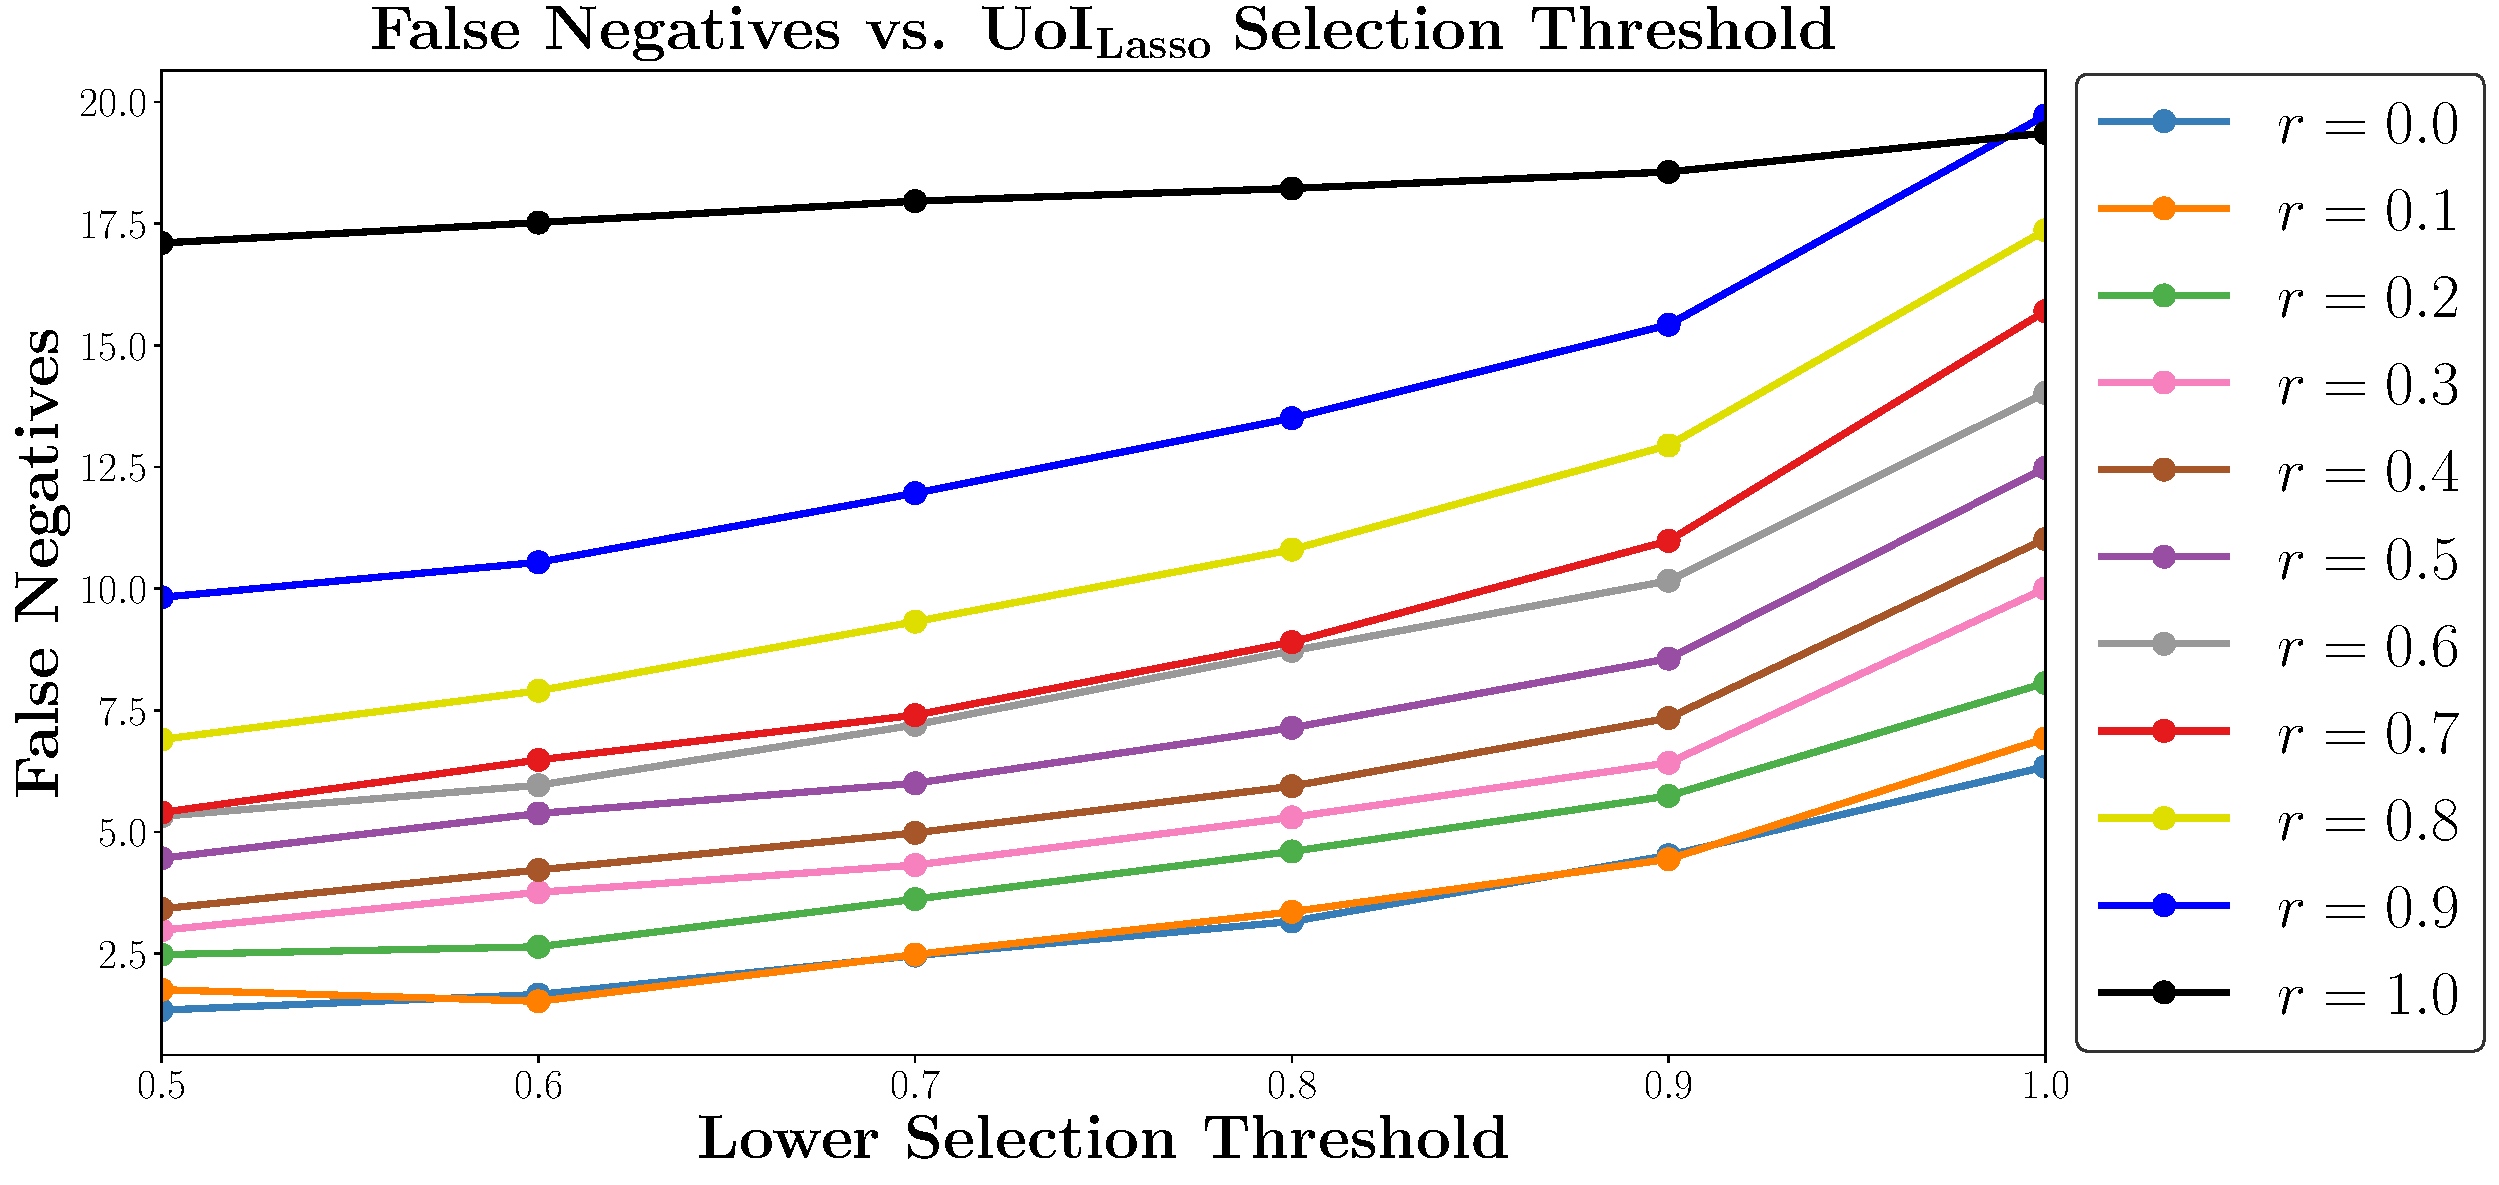
\includegraphics{img/exp1_fn_vs_lower_threshold.pdf}}
		\caption{False negatives vs. Lower selection threshold. Depicted are averages over 50 separate models. As we decrease the selection threshold, we select more variables and therefore observe fewer false negatives. Traditional UoI$_{\text{Lasso}}$ is given by $L_{f_s} = 1.0$ on the right hand side. For $r=1.0$, we see 20 false negatives, which makes sense: UoI$_{\text{Lasso}}$ will only select one variable among each of the five groups (setting the remaining 20 to zero).}
		\label{fig:exp1_fn-vs-thres}
	\end{figure}
	\begin{figure}[ht]
		\centering
		\scalebox{0.32}{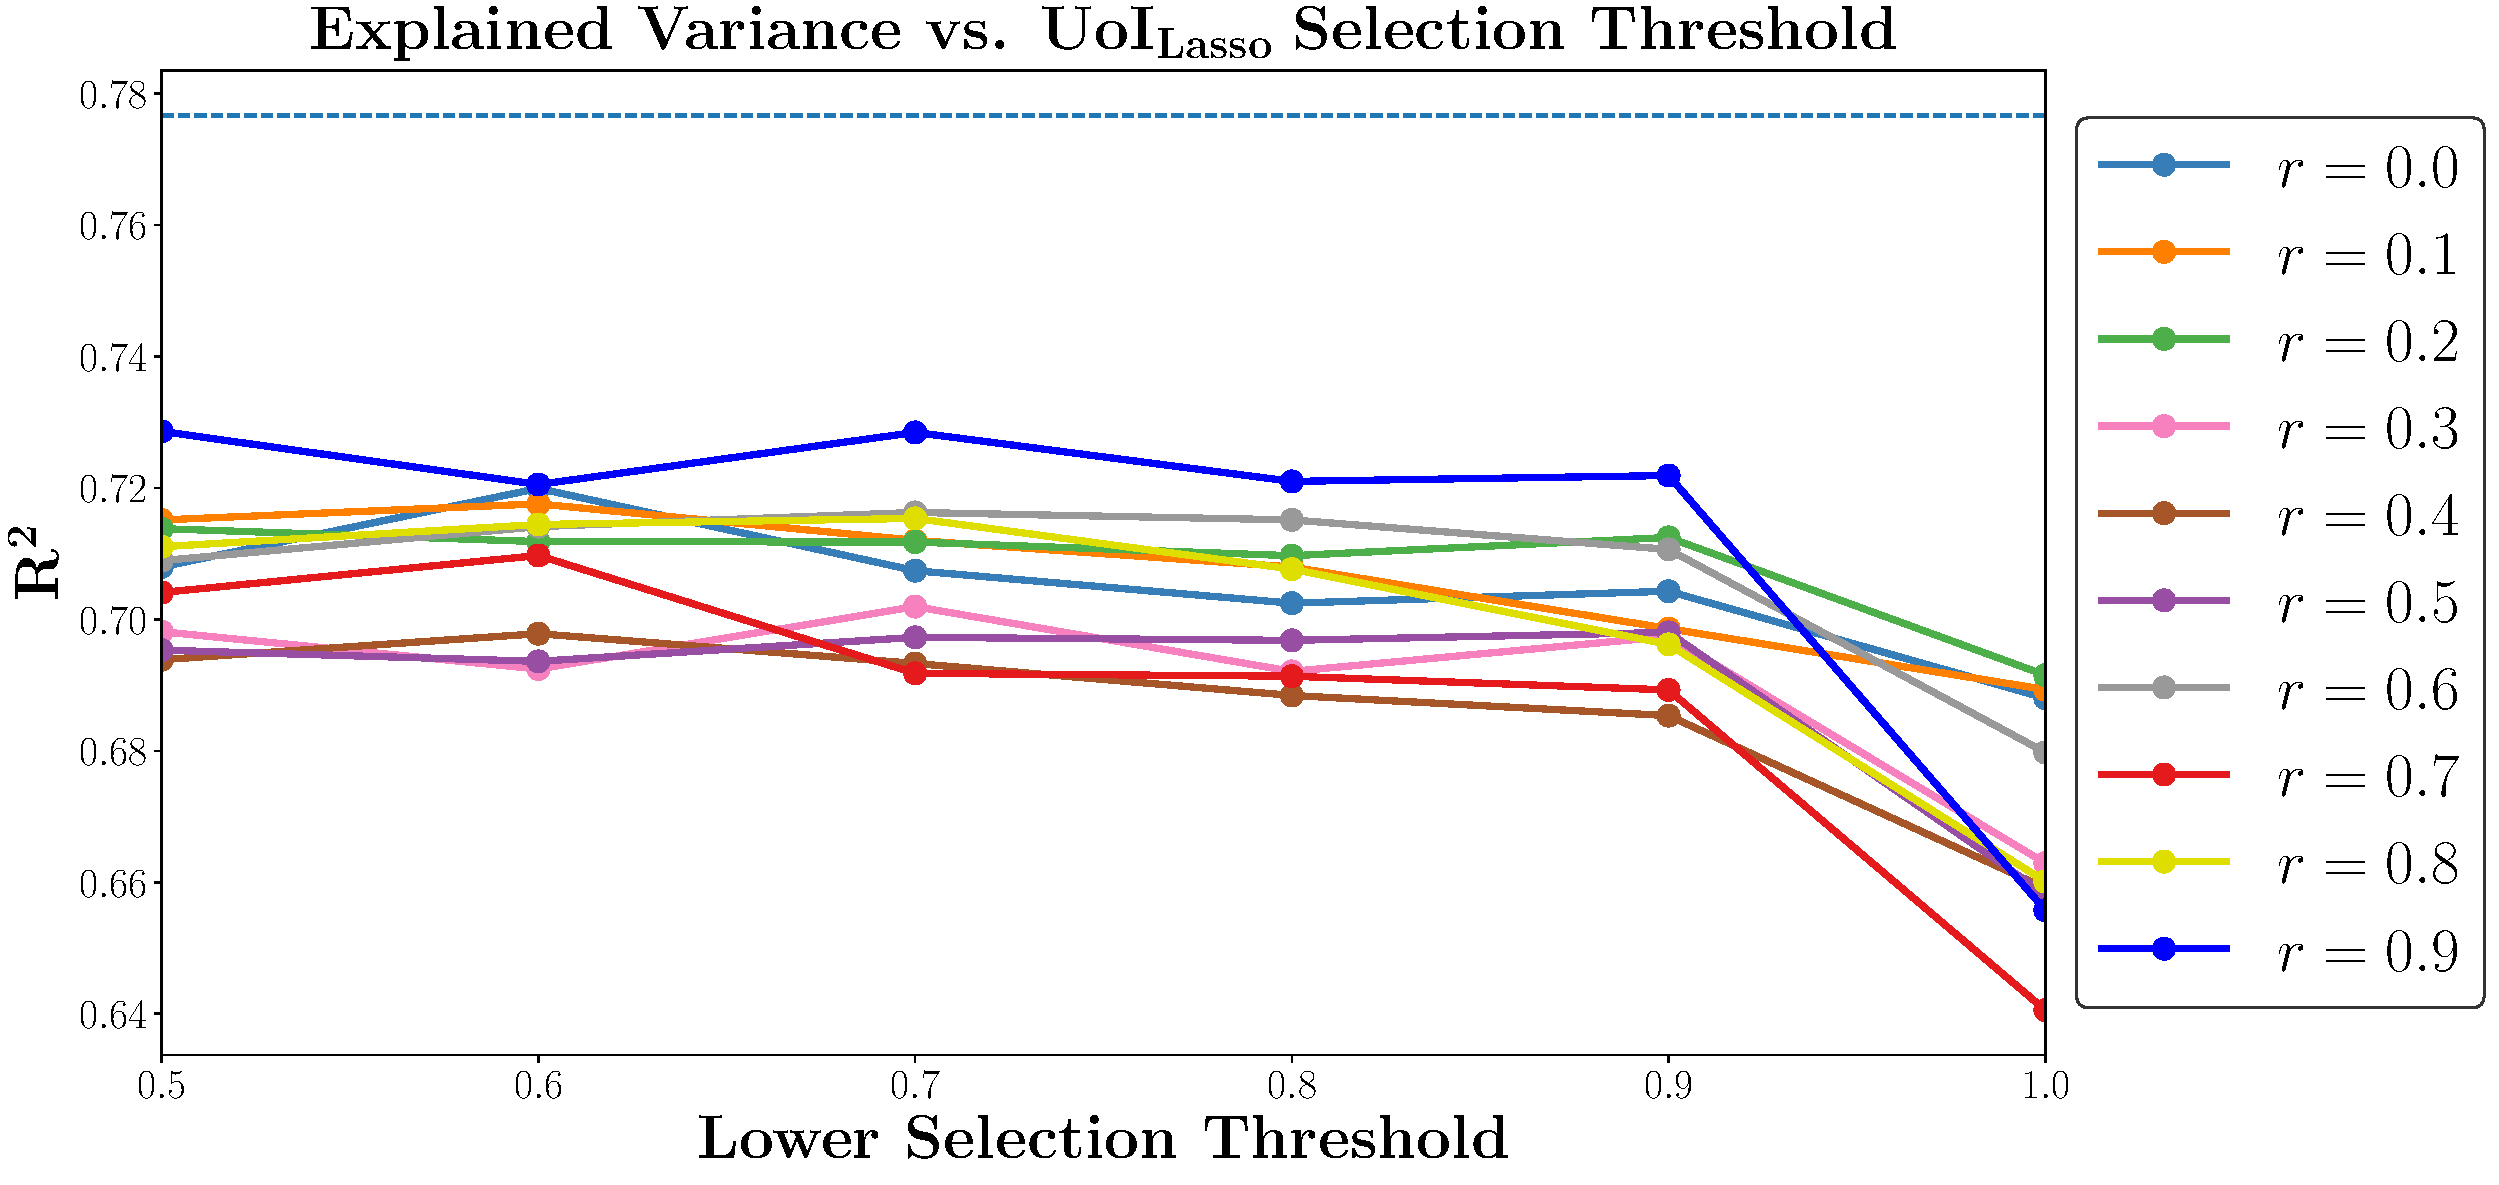
\includegraphics{img/exp1_r2_vs_lower_threshold.pdf}}
		\caption{Median explained variance over various lower selection thresholds. There is generally an increase in $R^2$ as $L_{f_s}$ is decreased. The dashed blue line indicates the median performance by the true parameters. Lastly, we did not include $r=1.0$ since the $R^2$ was poor.}
		\label{fig:exp1_r2-vs-thres}
	\end{figure}

\section{Experiment 2}
In experiment 1, we had no false positives since all parameters were included in the true model. This effectively corresponds to a sparsity of $s=1.$ In this experiment, we relaxed that sparsity constraint and allowed $s$ to vary from $0.1$ to $1.0$. We enforced sparsity uniformly across groups. For example, consider a model with $50$ features divided into $5$ groups of $10$ and a sparsity of $s=0.4$. Then, each group had $10 \times 0.4 = 4$ non-zero parameters, and there were $50\times 0.4 = 20 = 4\times 5$ non-zero parameters overall. 

In this experiment, we considered a $50$ dimensional feature vector consisting of $10$ groups of correlated features. We varied the within-group uniform correlation $r$, as before, but also varied the sparsity $s$. For each choice of $(r,s)$, we fit UoI$_{\text{Lasso}}$ with multiple lower selection thresholds (LSTs). Finally, as before, we performed this estimation procedure on 50 unique datasets over which we present aggregate results. Thus, there are three meaningful axes along which to evaluate the UoI performance. 

First, we can summarize the selection performance using false positives and false negatives with a plot inspired by ROC curves: we plot the false negative rate against the false positive rate for various choices of LST. This plot is shown in Figure \ref{fig:exp2-roc}, over multiple sparsities and across correlation values. When plotting the selection accuracies this way, it becomes easier to visualize what an optimal LST might be.

\begin{figure}[ht]
	\centering
	\scalebox{0.28}{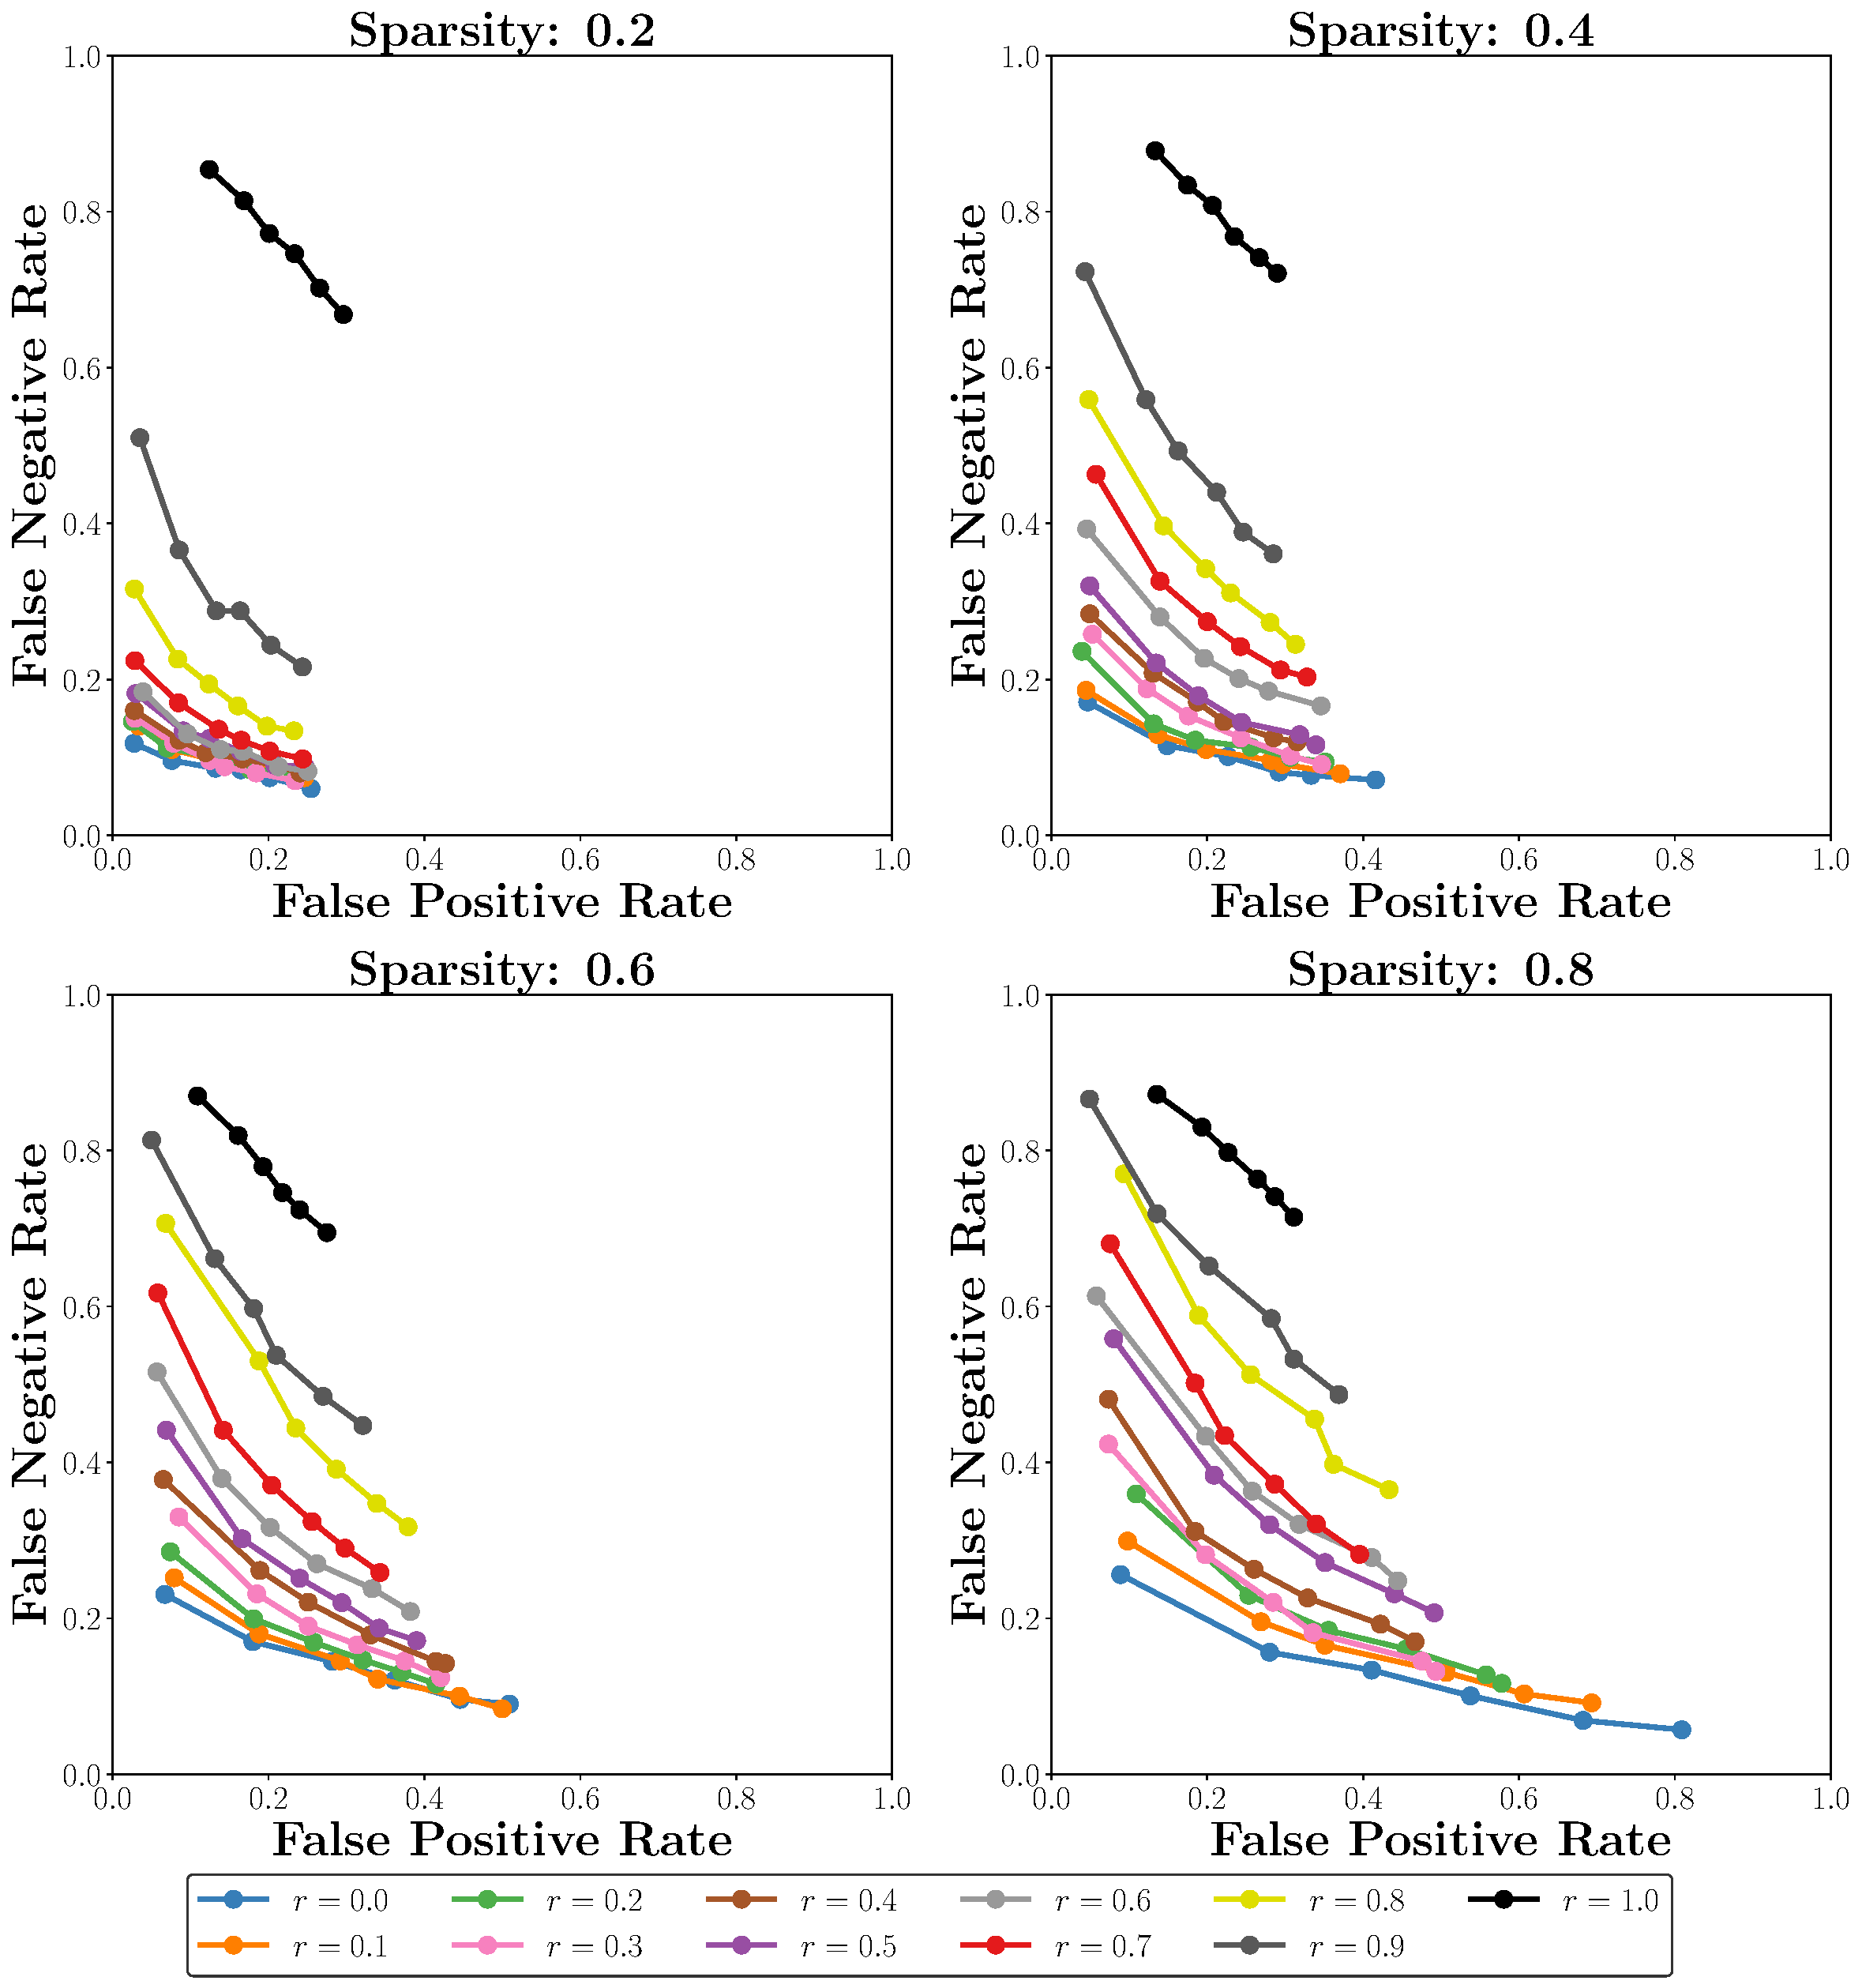
\includegraphics{img/exp2_roc.pdf}}
	\caption{False negative rate against false positive rate for different values of lower selection threshold in the UoI algorithm. Generally, larger false positive rates correspond to smaller LSTs.}
	\label{fig:exp2-roc}
\end{figure}

Next, we might ask if UoI$_{\text{Lasso}}$ is selecting representative parameters from each group. This becomes relevant for higher correlations, when it is possible that one parameter provides good prediction accuracy as a substitute for the entire group. We plot the number of parameters selected per group across datasets for a variety of sparsities and correlations in Figure \ref{fig:exp2-n-per-group}.
\begin{figure}[H]
	\centering
	\scalebox{0.25}{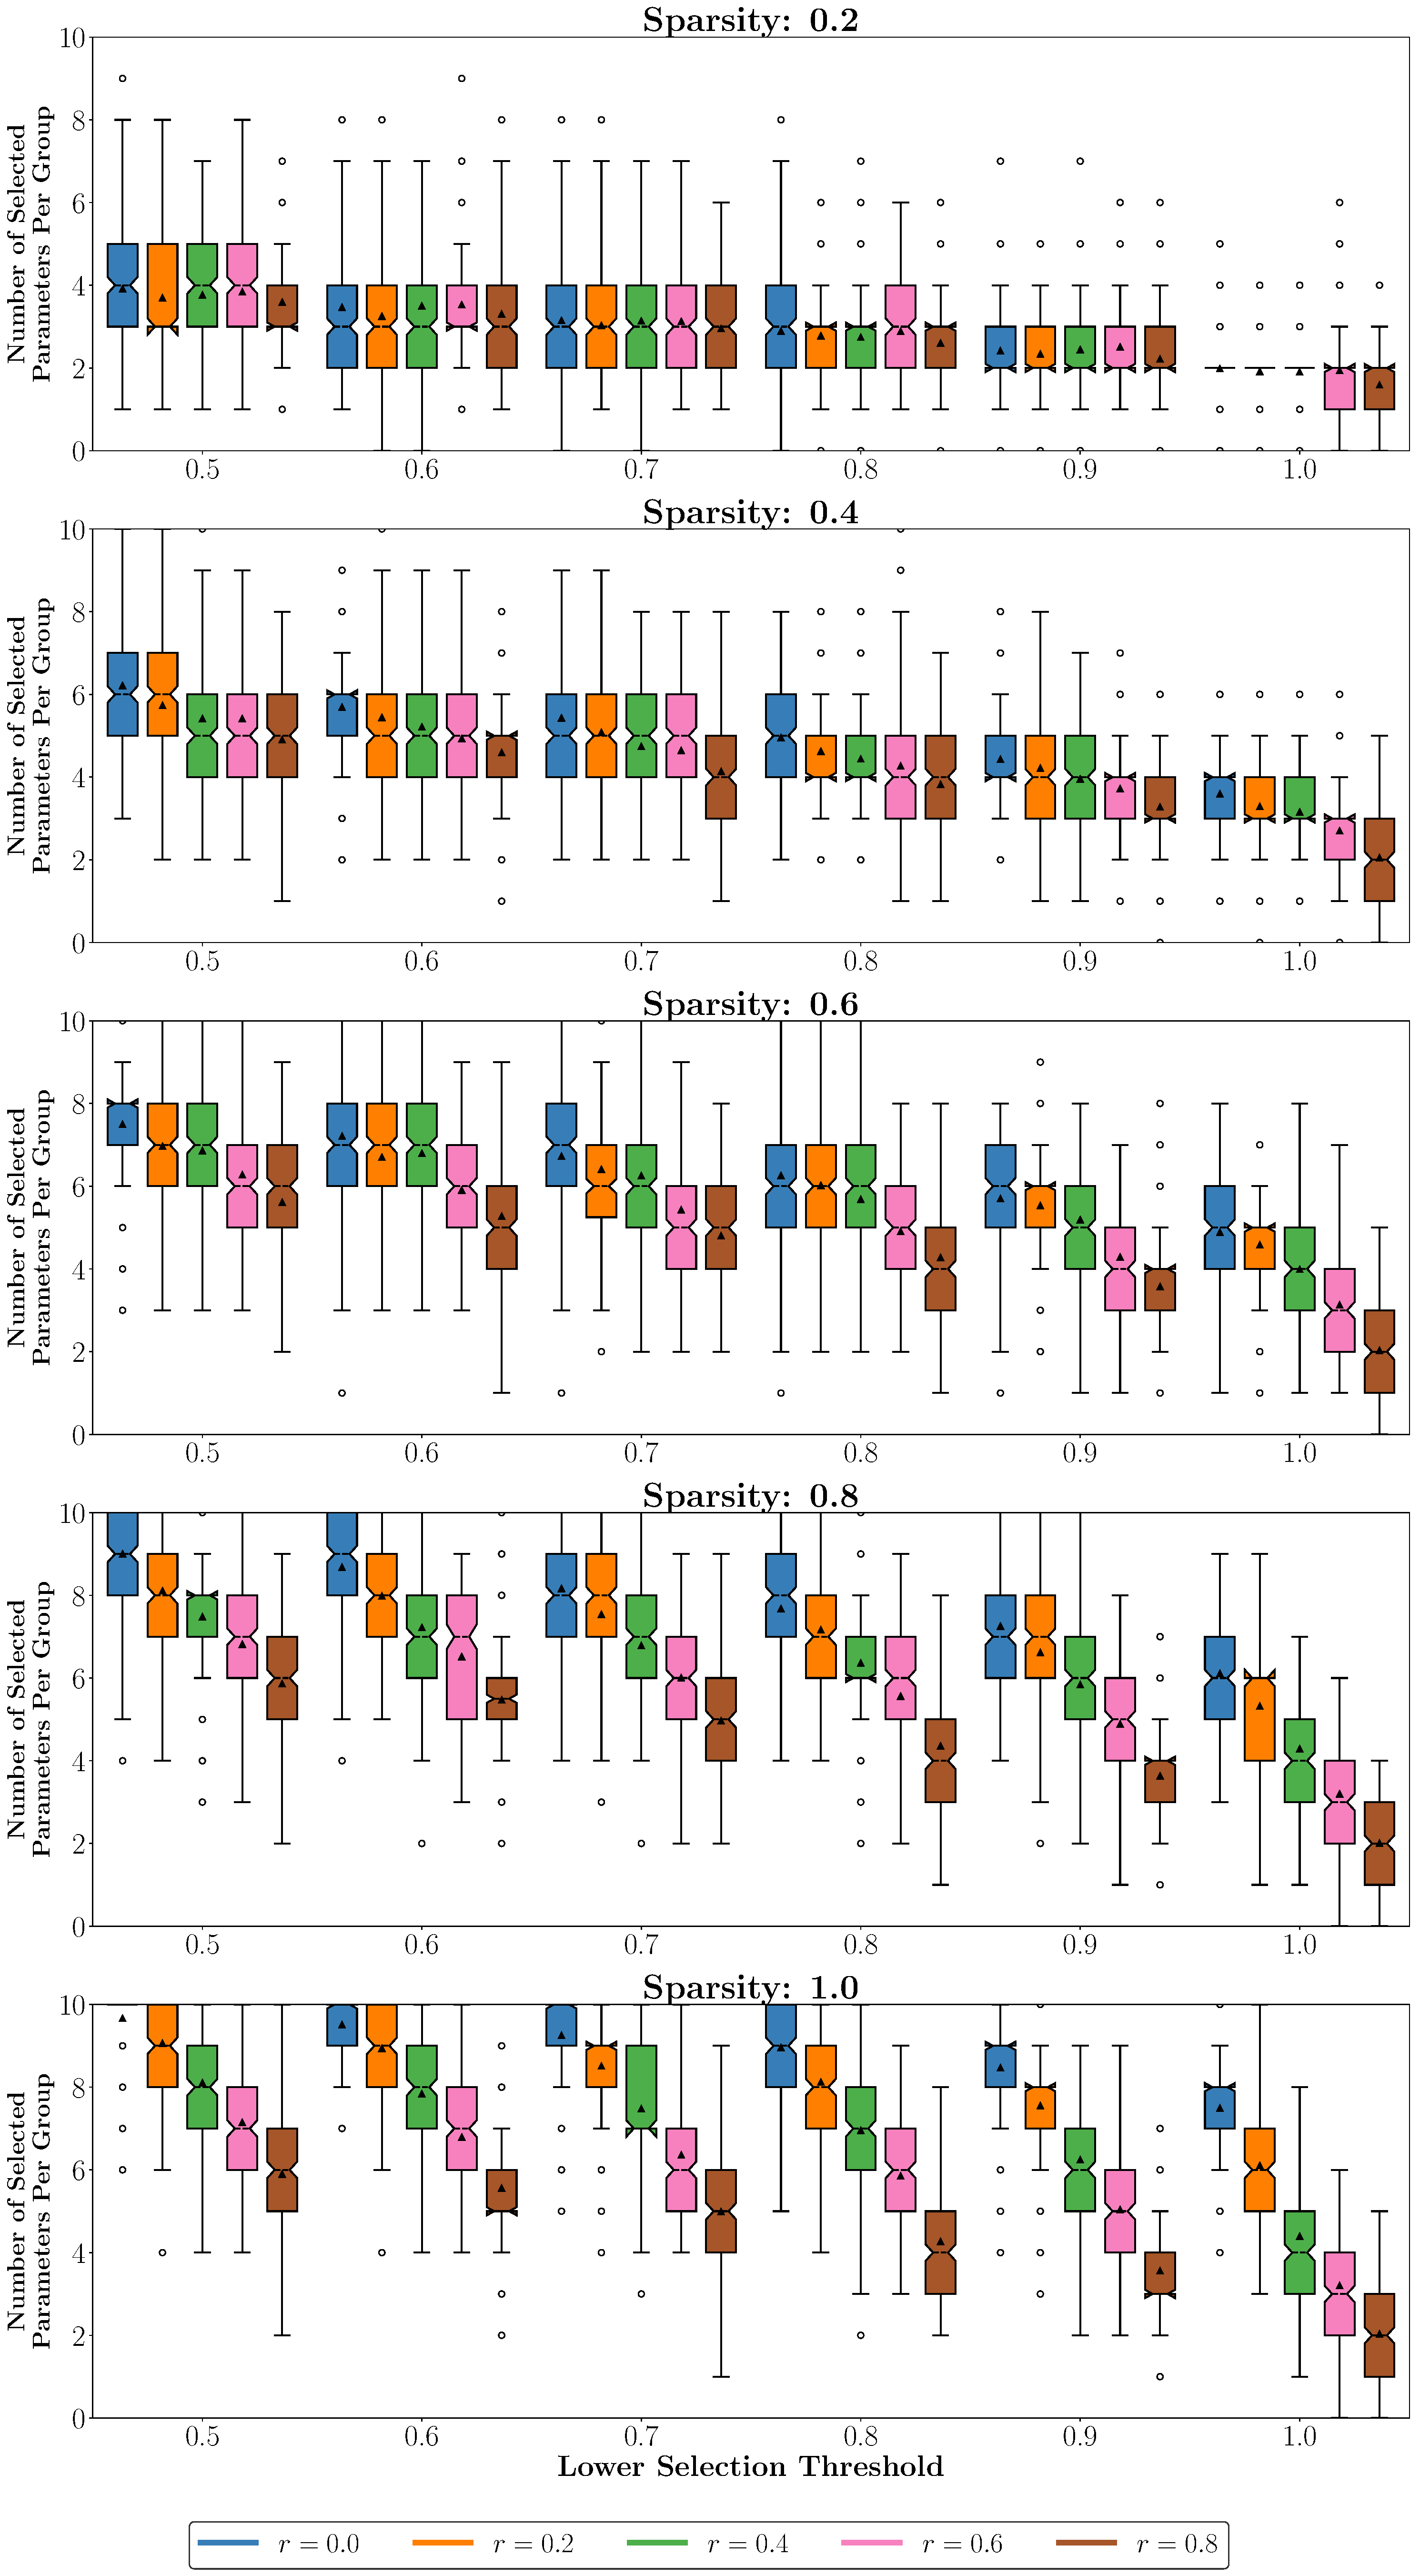
\includegraphics{img/exp2_n_per_group.pdf}}
	\caption{Number of parameters selected per group. Boxplots are taken over all groups and all datasets (thus, there are $50\times 5=250$ points in each boxplot).}
	\label{fig:exp2-n-per-group}
\end{figure}

Thus, it is clear that UoI$_{\text{Lasso}}$ is selecting less parameters both as the LST increases and as the correlation increases. This implies an increase in false negatives. Thus, the next natural question to ask if: given an increase in false negatives, which parameters are getting selected out? Our expectation is that the smaller parameters would be selected out. We plot the average magnitude of false negatives as a function of sparsity, LST, and correlation in Figure \ref{fig:exp2-mag-fn}. Immediately, we see that the average magnitude has a very weak dependence on LST. Furthermore, the average magnitude of false negatives increases with correlation, while the shape of the distribution changes with sparsity.

\begin{figure}[H]
	\centering
	\scalebox{0.24}{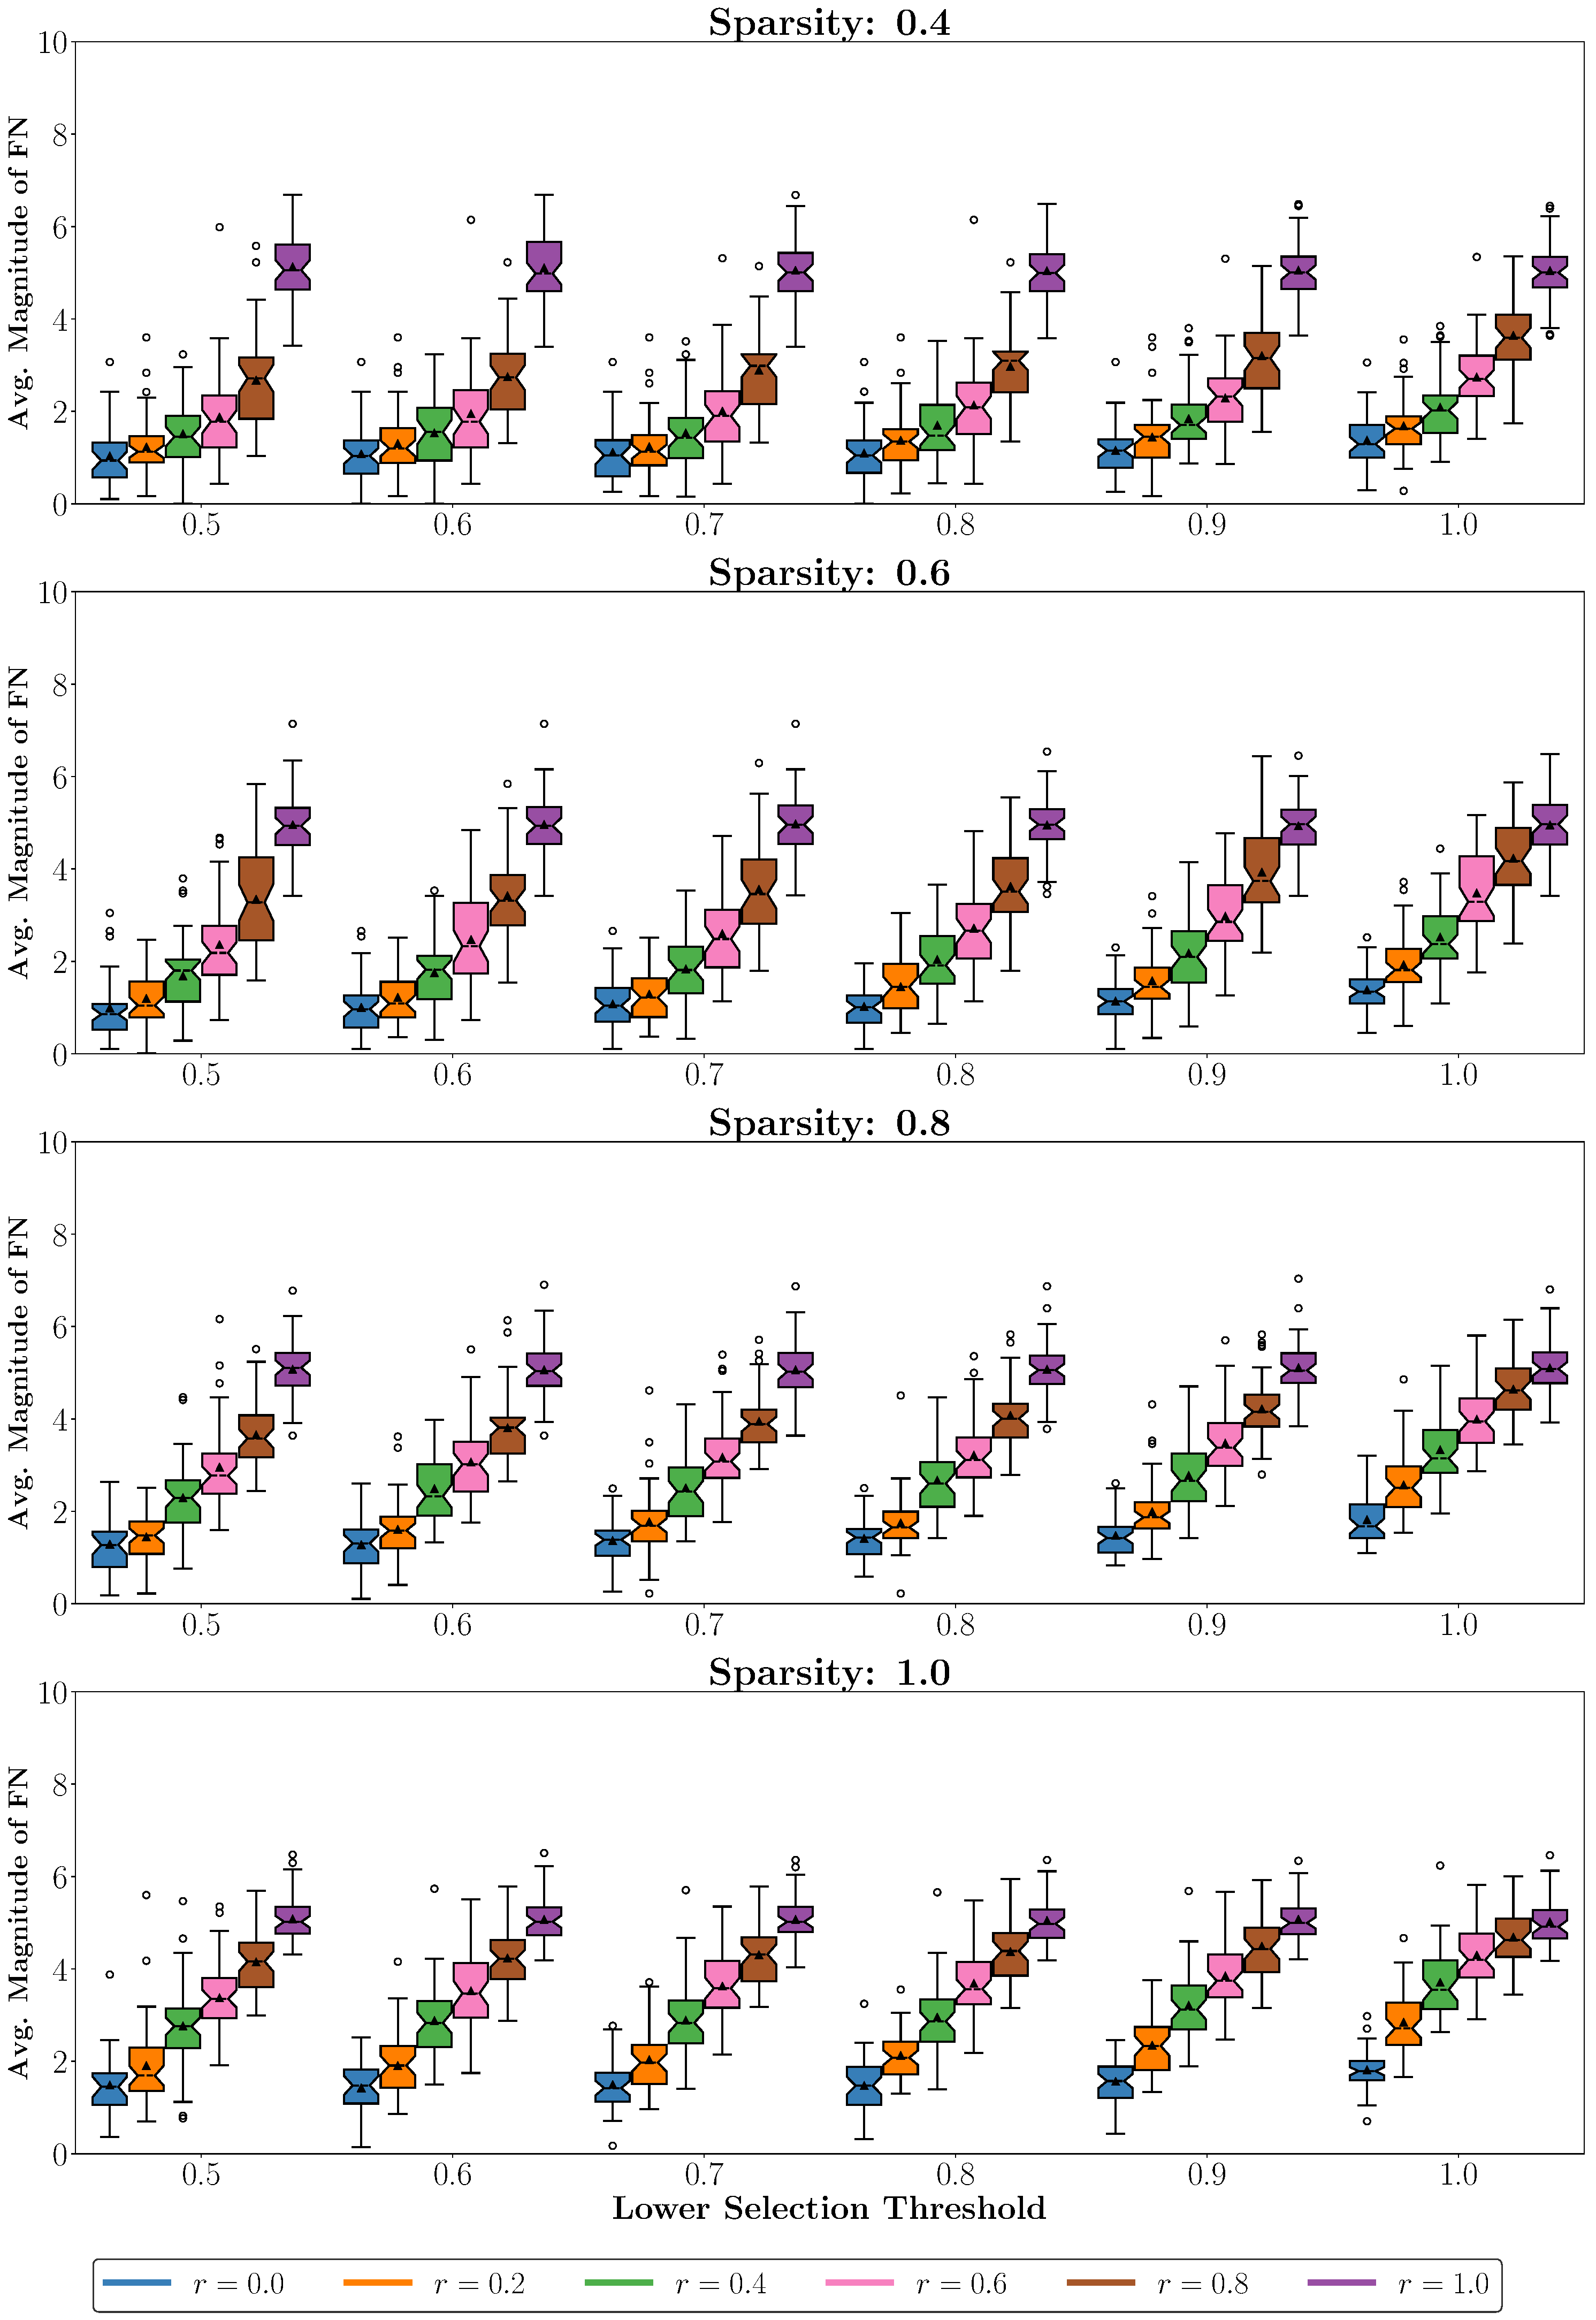
\includegraphics{img/exp2_mag_fn.pdf}}
	\caption{Average magnitude of false negatives. Boxplots contain the average magnitude of the true parameters which were falsely selected out by UoI$_{\text{Lasso}}$, taken across datasets. }
	\label{fig:exp2-mag-fn}
\end{figure}

Since the boxplots above are taken across separate instantiations of the problem, with completely different $\beta$ values, the actual spread of the boxplot is somewhat meaningless. To be clear, one instantiation might have artificially inflated values of $\beta$, thereby artificially increasing the average magnitude of the false negatives. Thus, to normalize over instantiations, we calculated the scaled false negative rate, given by
\begin{align}
	\text{scaled false negative rate} &= \frac{\sum_{j \in \text{FN}} |\beta_j|}{\sum_{i=1}^{10} |\beta_i|},
\end{align}
i.e. the $\ell_1$-norm of the true parameters selected out by the algorithm divided by the $\ell_1$-norm of the entire vector of parameters. The difficult of this parameter is that a low value might conflate both selecting out small values of $\beta_i$ or a low false negative rate.

\begin{figure}[H]
	\centering
	\scalebox{0.23}{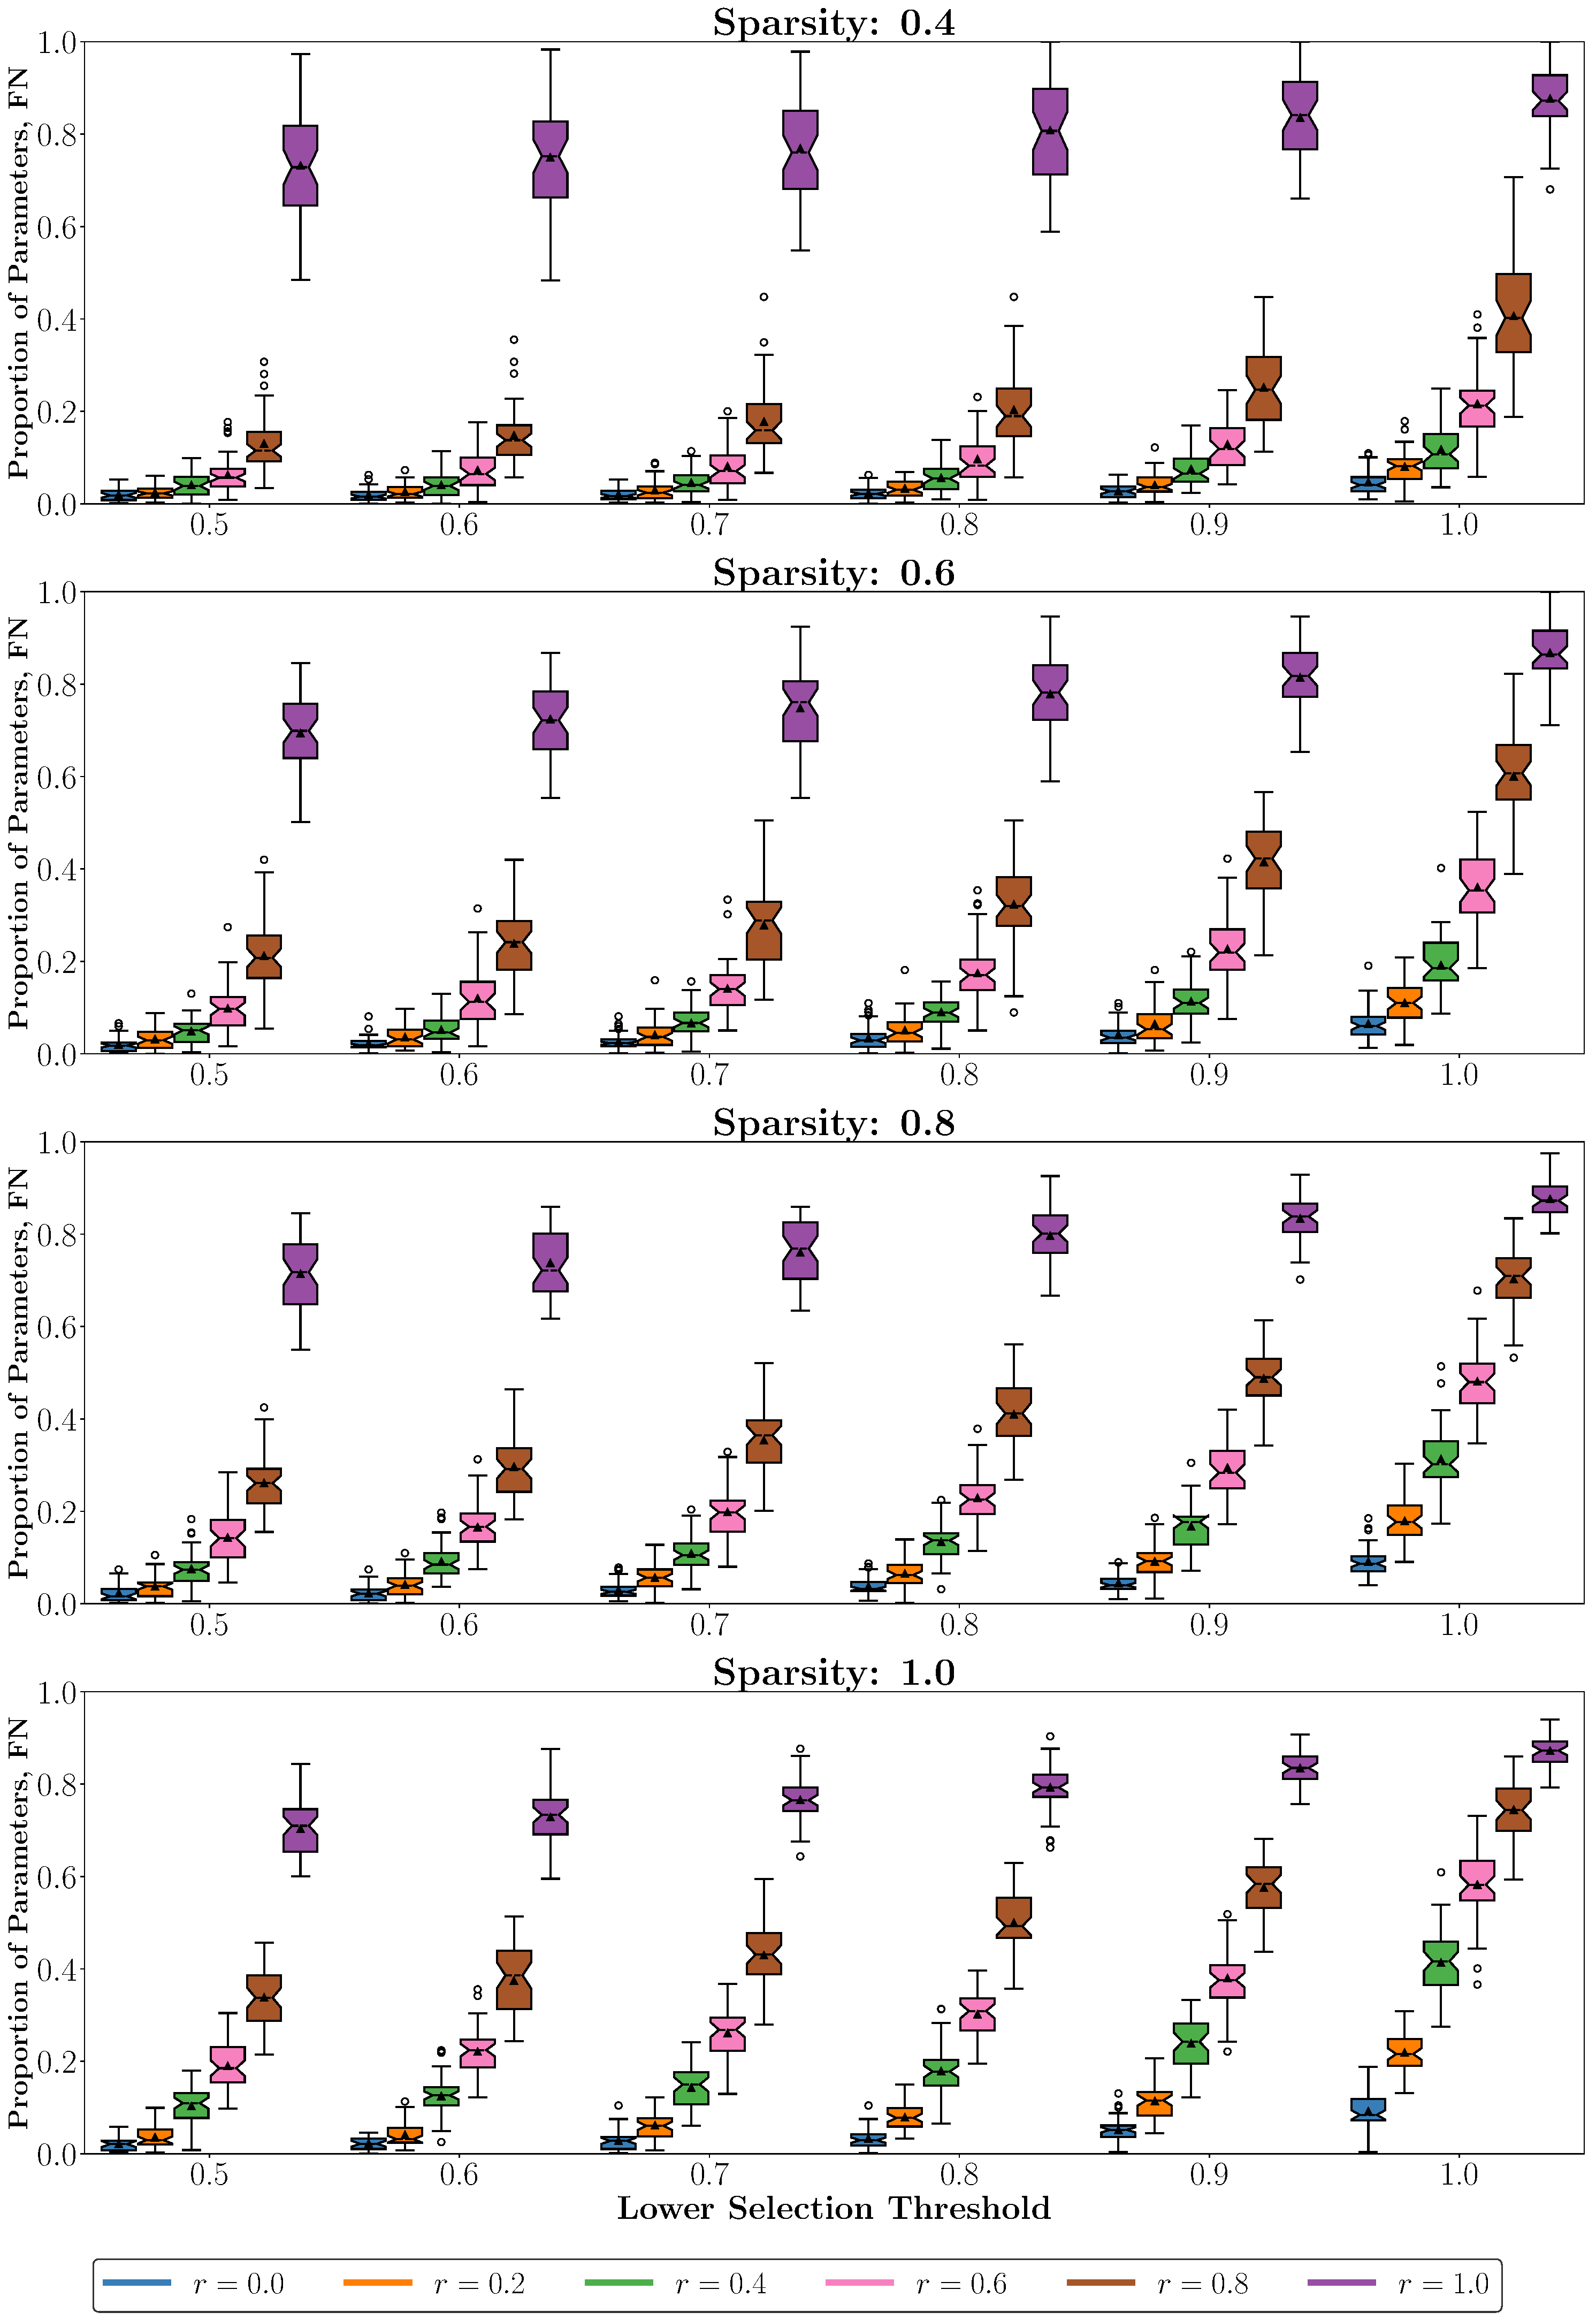
\includegraphics{img/exp2_mag_fn_scaled.pdf}}
	\caption{Average magnitude of false negatives. Boxplots contain the average magnitude of the true parameters which were falsely selected out by UoI$_{\text{Lasso}}$, taken across datasets. }
	\label{fig:exp2-mag-fn}
\end{figure}

The above two plots exhibit a weak dependence on LST. Thus, a 2d surface plot between sparsity and correlation would be useful to examine. The plots are shown in Figure \ref{fig:exp2-mag-fn-surface}. 

\begin{figure}[H]
	\centering
	\scalebox{0.40}{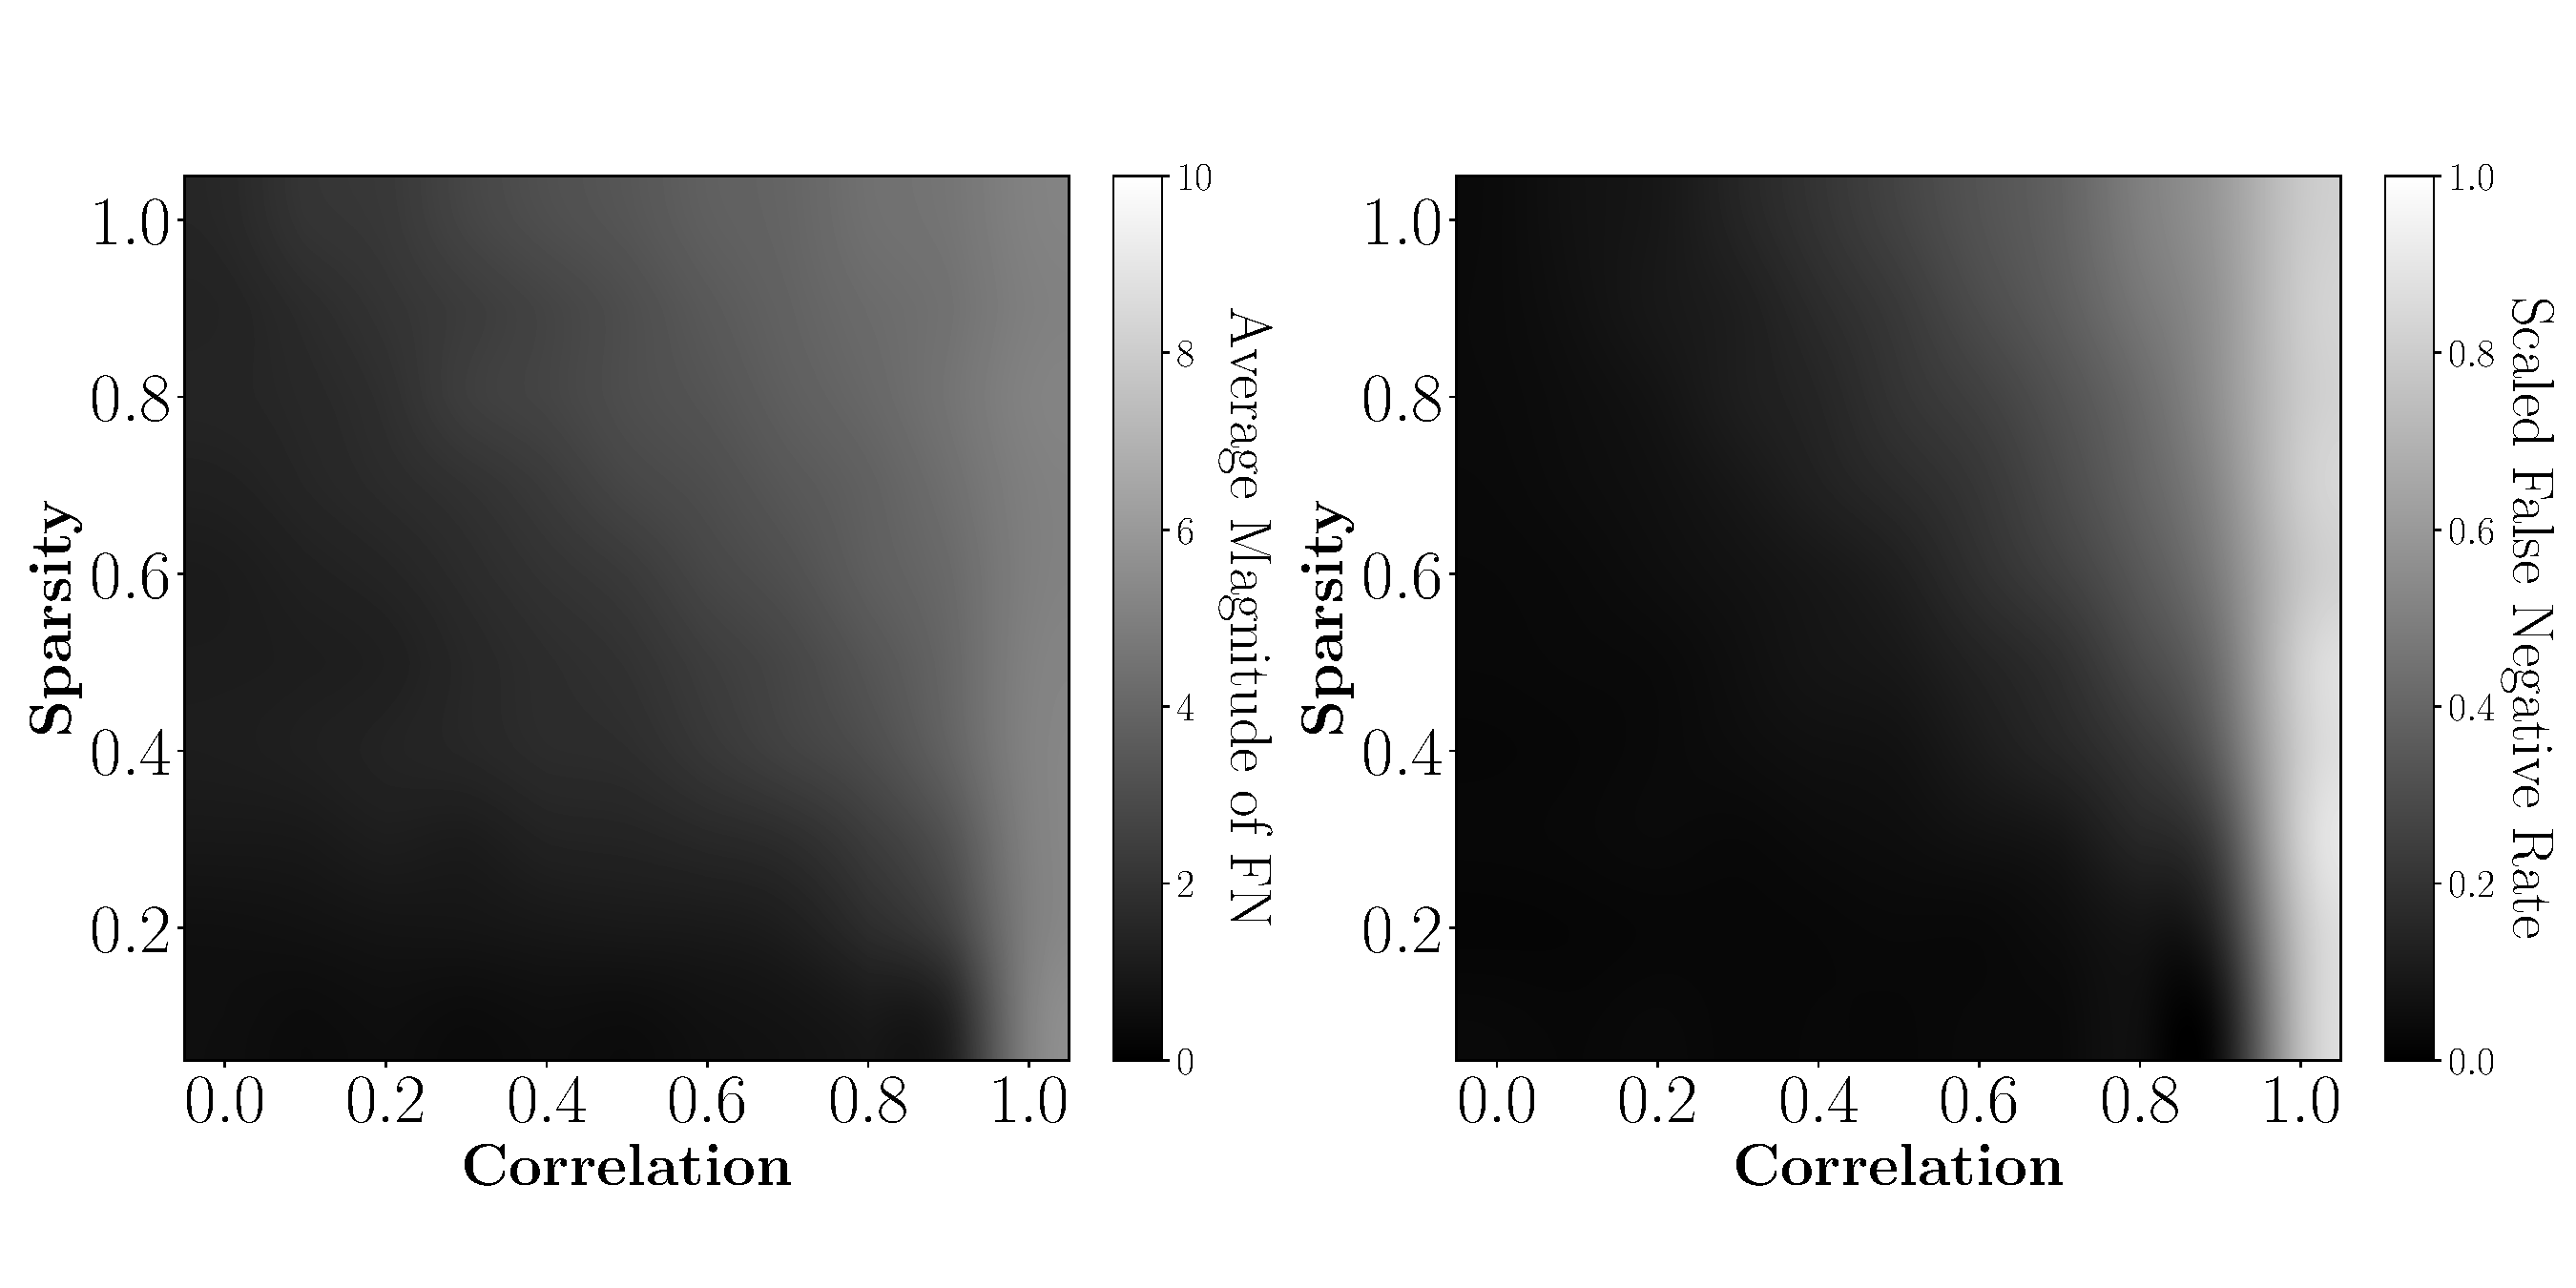
\includegraphics{img/exp2_mag_fn_2d.pdf}}
	\caption{Surface plots of the previous two plots, with varying sparsity and correlation. Shown are averages over LST and the 50 instantiations. The general trends are similar as before:an increase in correlation and an increase in sparsity result in larger values of both quantities.}
	\label{fig:exp2-mag-fn-surface}
\end{figure}

Lastly, we consider \textit{selection accuracy per group}. This is a useful quantity to examine because the selection accuracy for an entire parameter vector will not be the same as the average of selection accuracies across groups (unlike false positives and false negatives). Thus, in Figure \ref{fig:exp2-sel-per-group}, we examine how LST, correlation, and sparsity impact the selection accuracy per group.  

There are a couple takeaways from the figure. First, sparsity is important: a smaller sparsity implies that the correlation will have a minimal impact on the optimal choice of LST. Next, just by eyeballing the figure, a LST of 0.7 is a generally optimal choice for any choice of correlation and sparsity. 

\begin{figure}[H]
	\centering
	\scalebox{0.25}{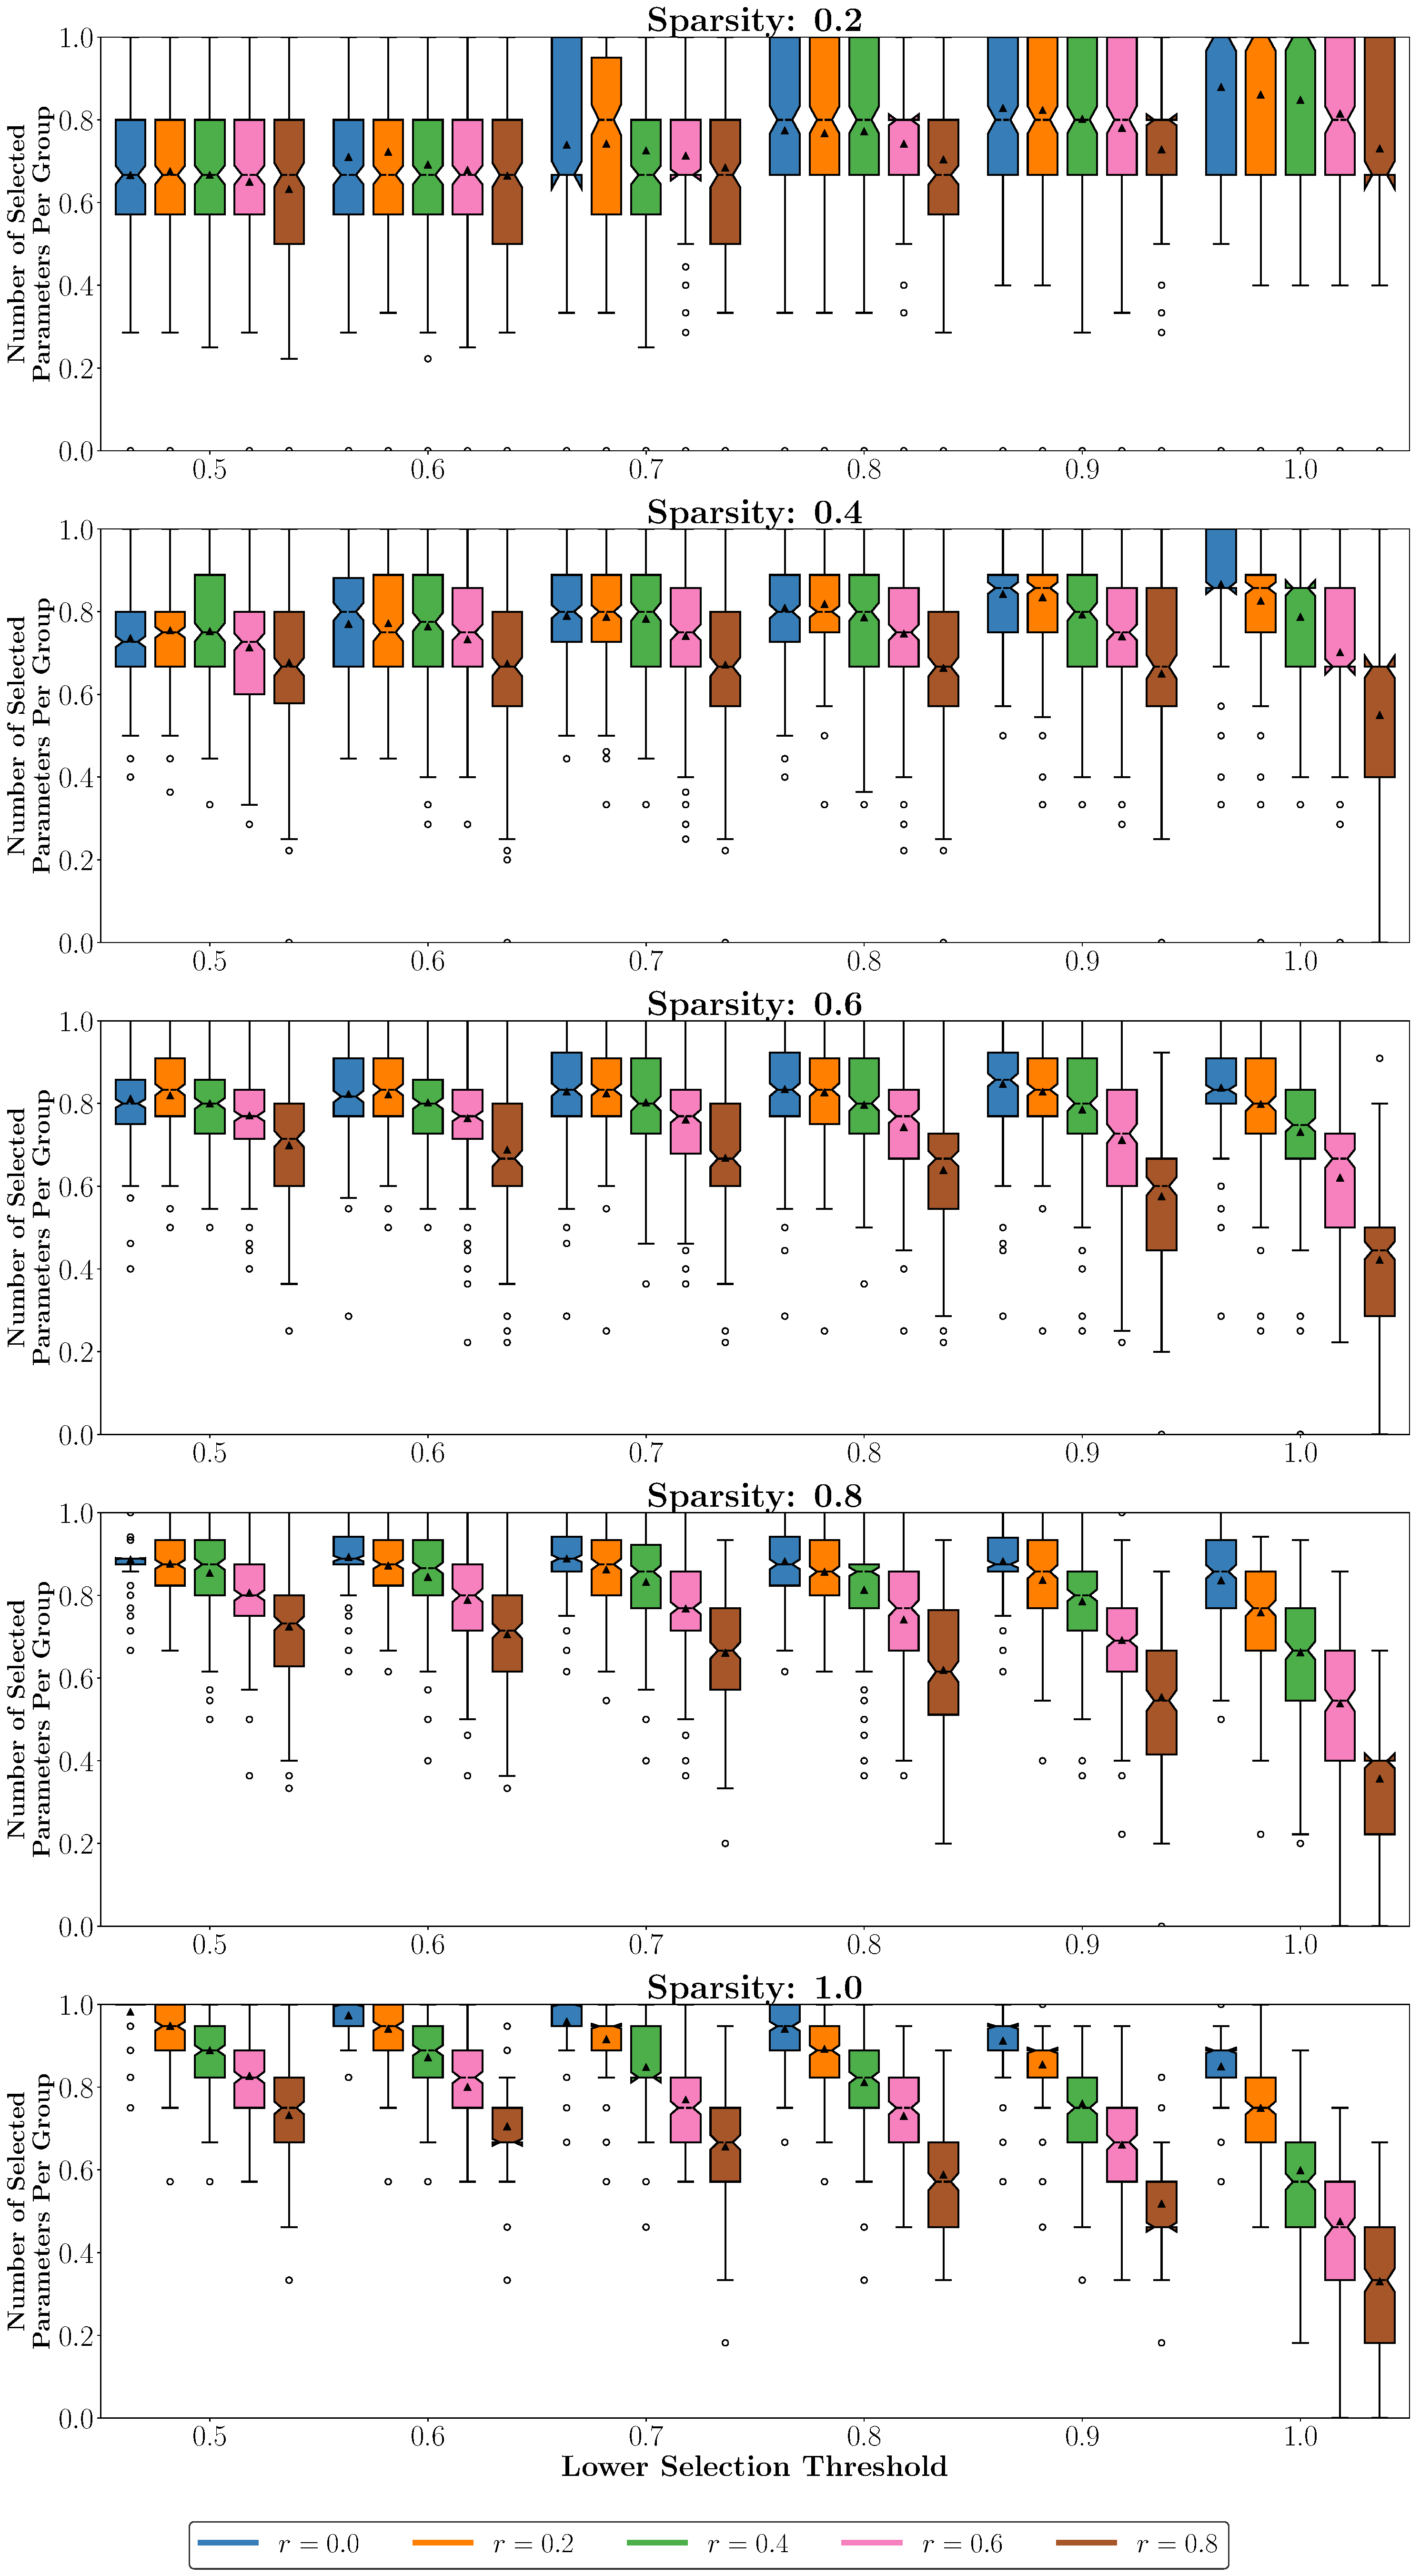
\includegraphics{img/exp2_sel_per_group.pdf}}
	\caption{Selection accuracy per group. Boxplots are selection accuracies for each group in a given feature vector, across all 50 datasets. Thus, they consist of $50\times 5 = 250$ points each.}
	\label{fig:exp2-sel-per-group}
\end{figure}

\section{Experiment 3}
In the previous experiments, we considered groups of correlated regressors. There existed no correlations between groups, however, which allowed the covariance matrix to take on a block-diagonal structure. In this experiment, we instead allow correlations to exist across all regressors with the magnitude set by a distance metric. The distance metric operated on the space of indices. Thus, for regressor $X_i$ and $X_j$ (with respective parameters $\beta_i$ and $\beta_j$), the correlation between them was 
\begin{align}
	\text{corr}(X_i, X_j) &= \exp\left(-\frac{|i-j|}{L}\right). \label{eqn:corr-falloff}
\end{align}
Equation \ref{eqn:corr-falloff} actually specifies the entire correlation matrix, as it ensures all diagonal terms are set to one. Thus, the hyperparameter $L$ dictates how fast correlations fall off. If $L$ is small, only regressors close to each other are correlated; if $L$ is large, then large correlations will exist across the matrix. 

Thus, while the previous formulation specified the correlation uniformly applied within in group ($r$), this formulation specifies how quickly correlations deteriorate ($L$). Once again, we enforce sparsity $s$, but now we make no restrictions on which parameters are zero (before, we enforced sparsity uniformly across groups). We once again assess how UoI$_{\text{Lasso}}$ performs with various choices of LST across 50 different instantiations of model. There are, as before, 3 dimensions of interest over which to evaluate performance: fall-off $L$, sparsity $s$, and LST. We can first examine the performance of UoI$_{\text{Lasso}}$ as LST is varied with a similar ROC plot as in Experiment 2.
\begin{figure}[H]
	\centering
	\scalebox{0.30}{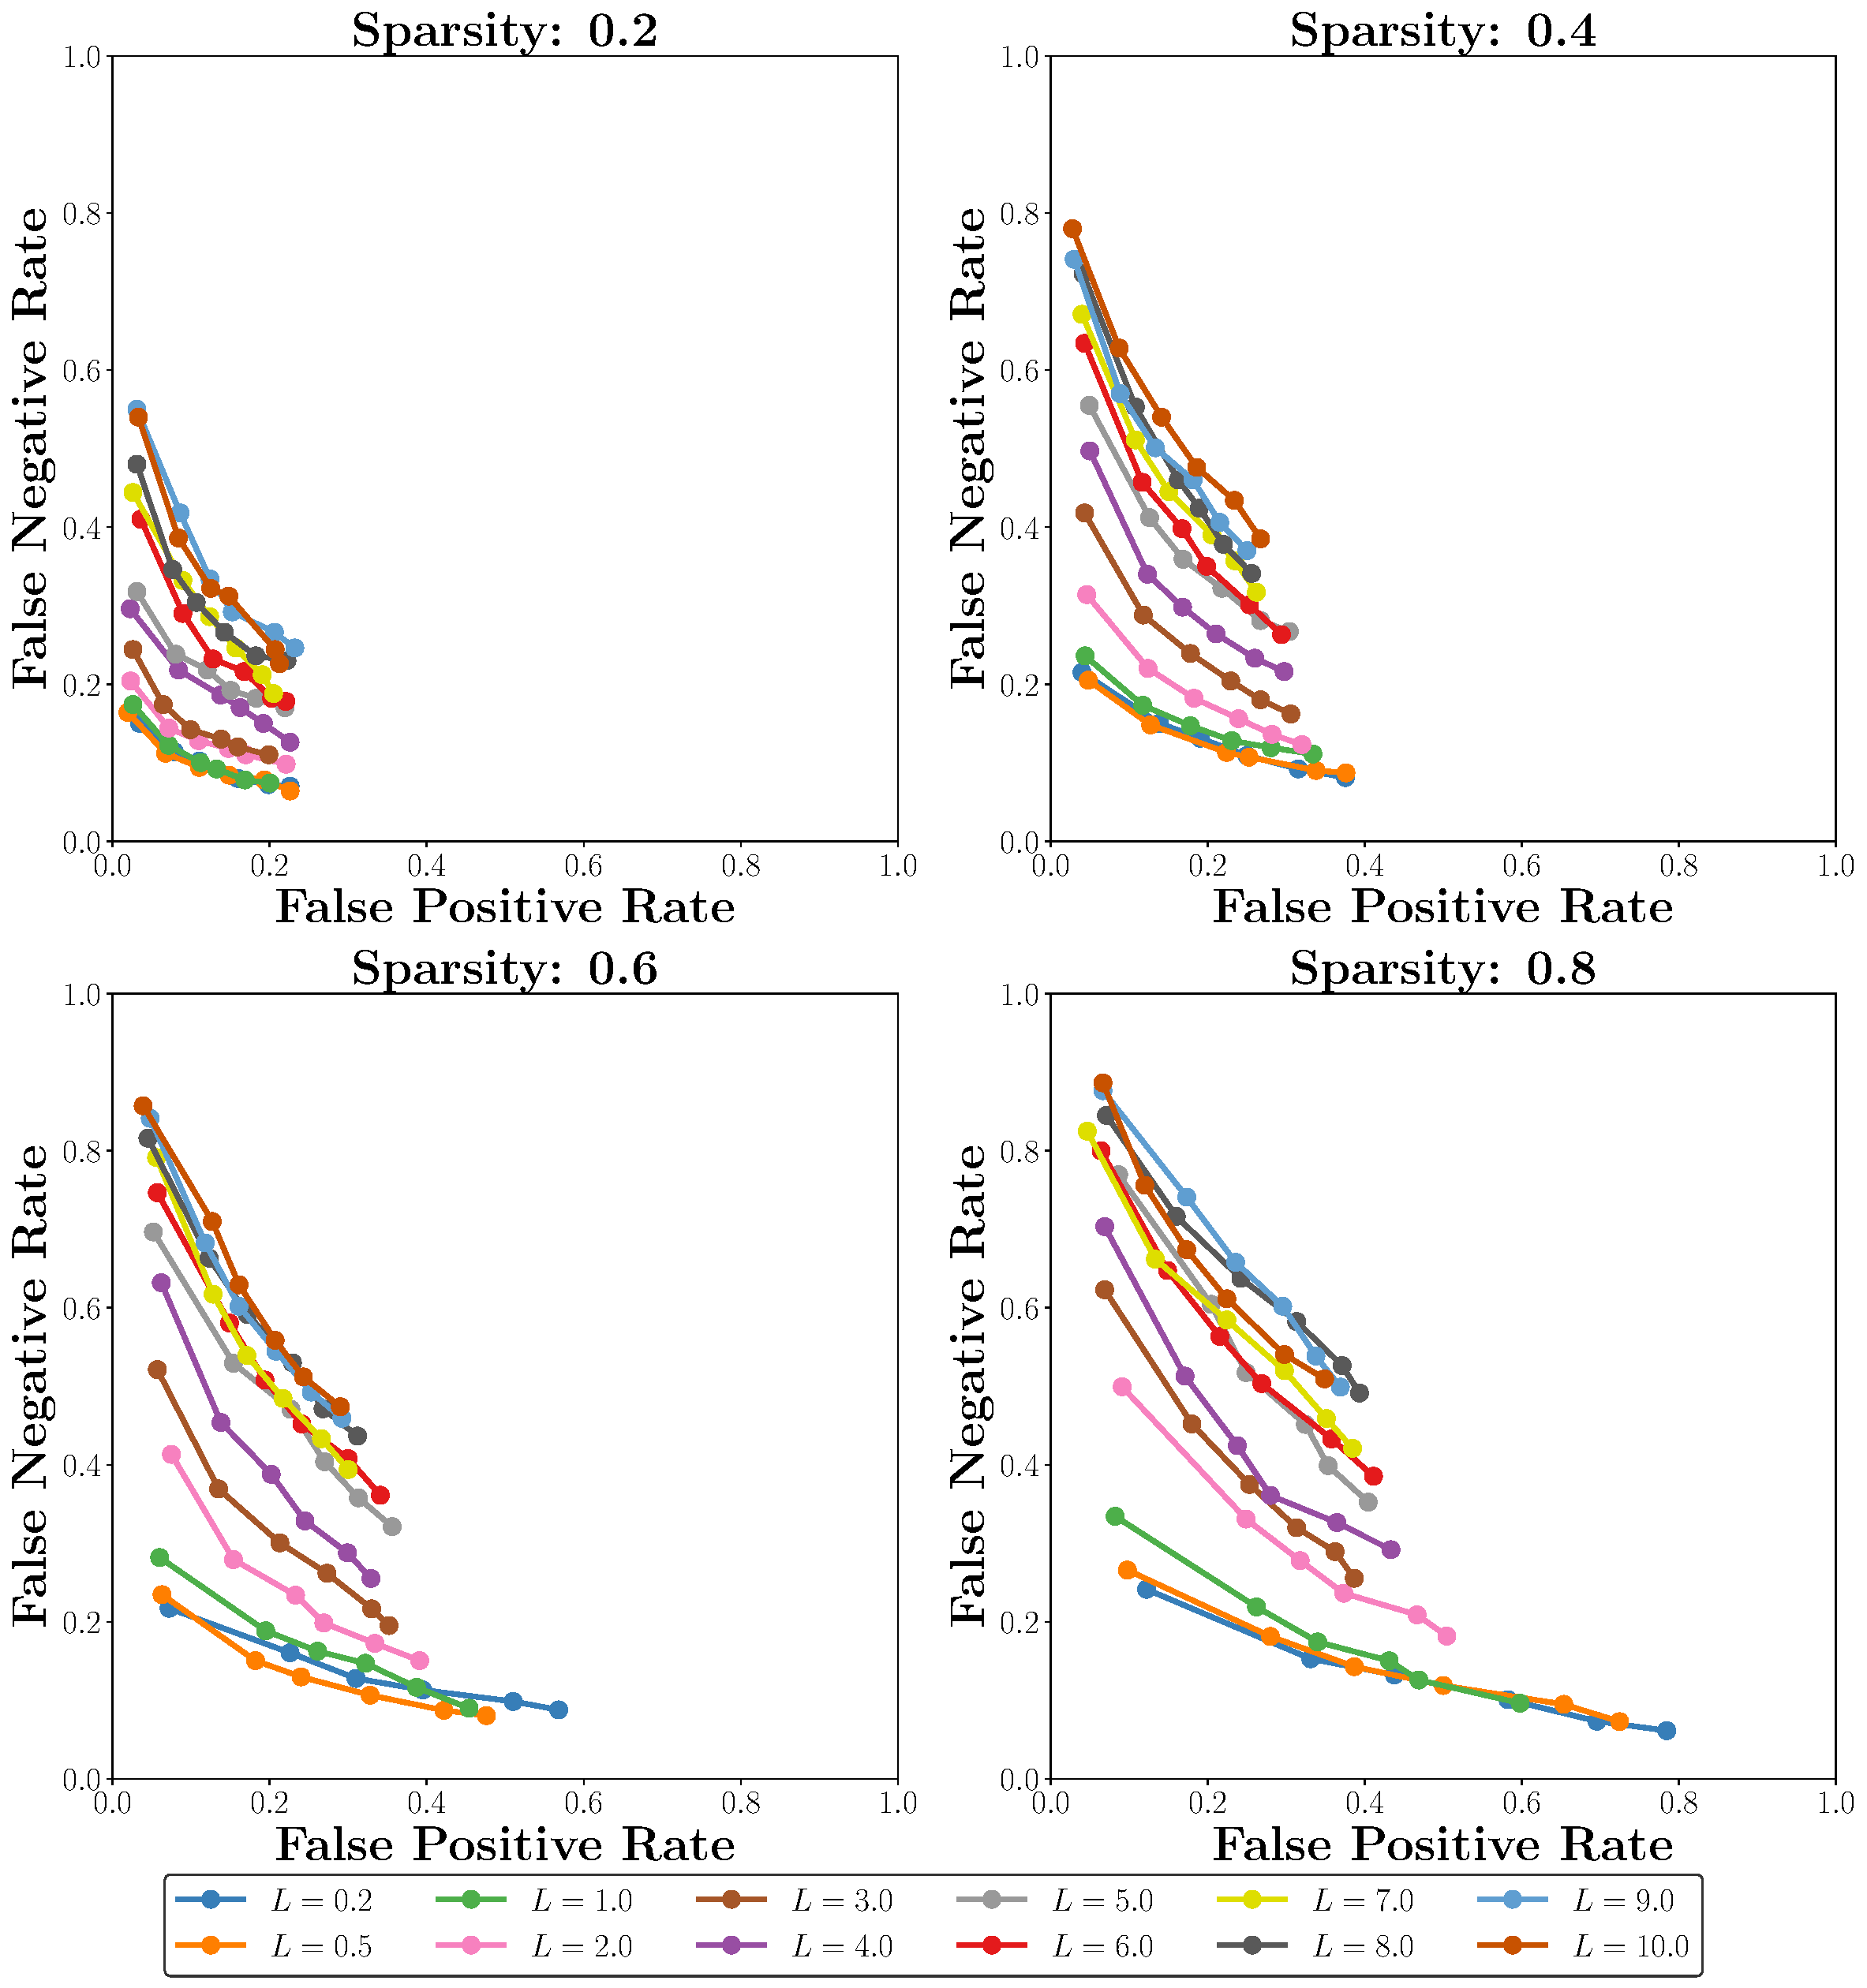
\includegraphics{img/exp3_roc.pdf}}
	\caption{FNR vs. FPR over various choices of LST.}
	\label{fig:exp3-roc}
\end{figure}

\begin{figure}[H]
	\centering
	\scalebox{0.30}{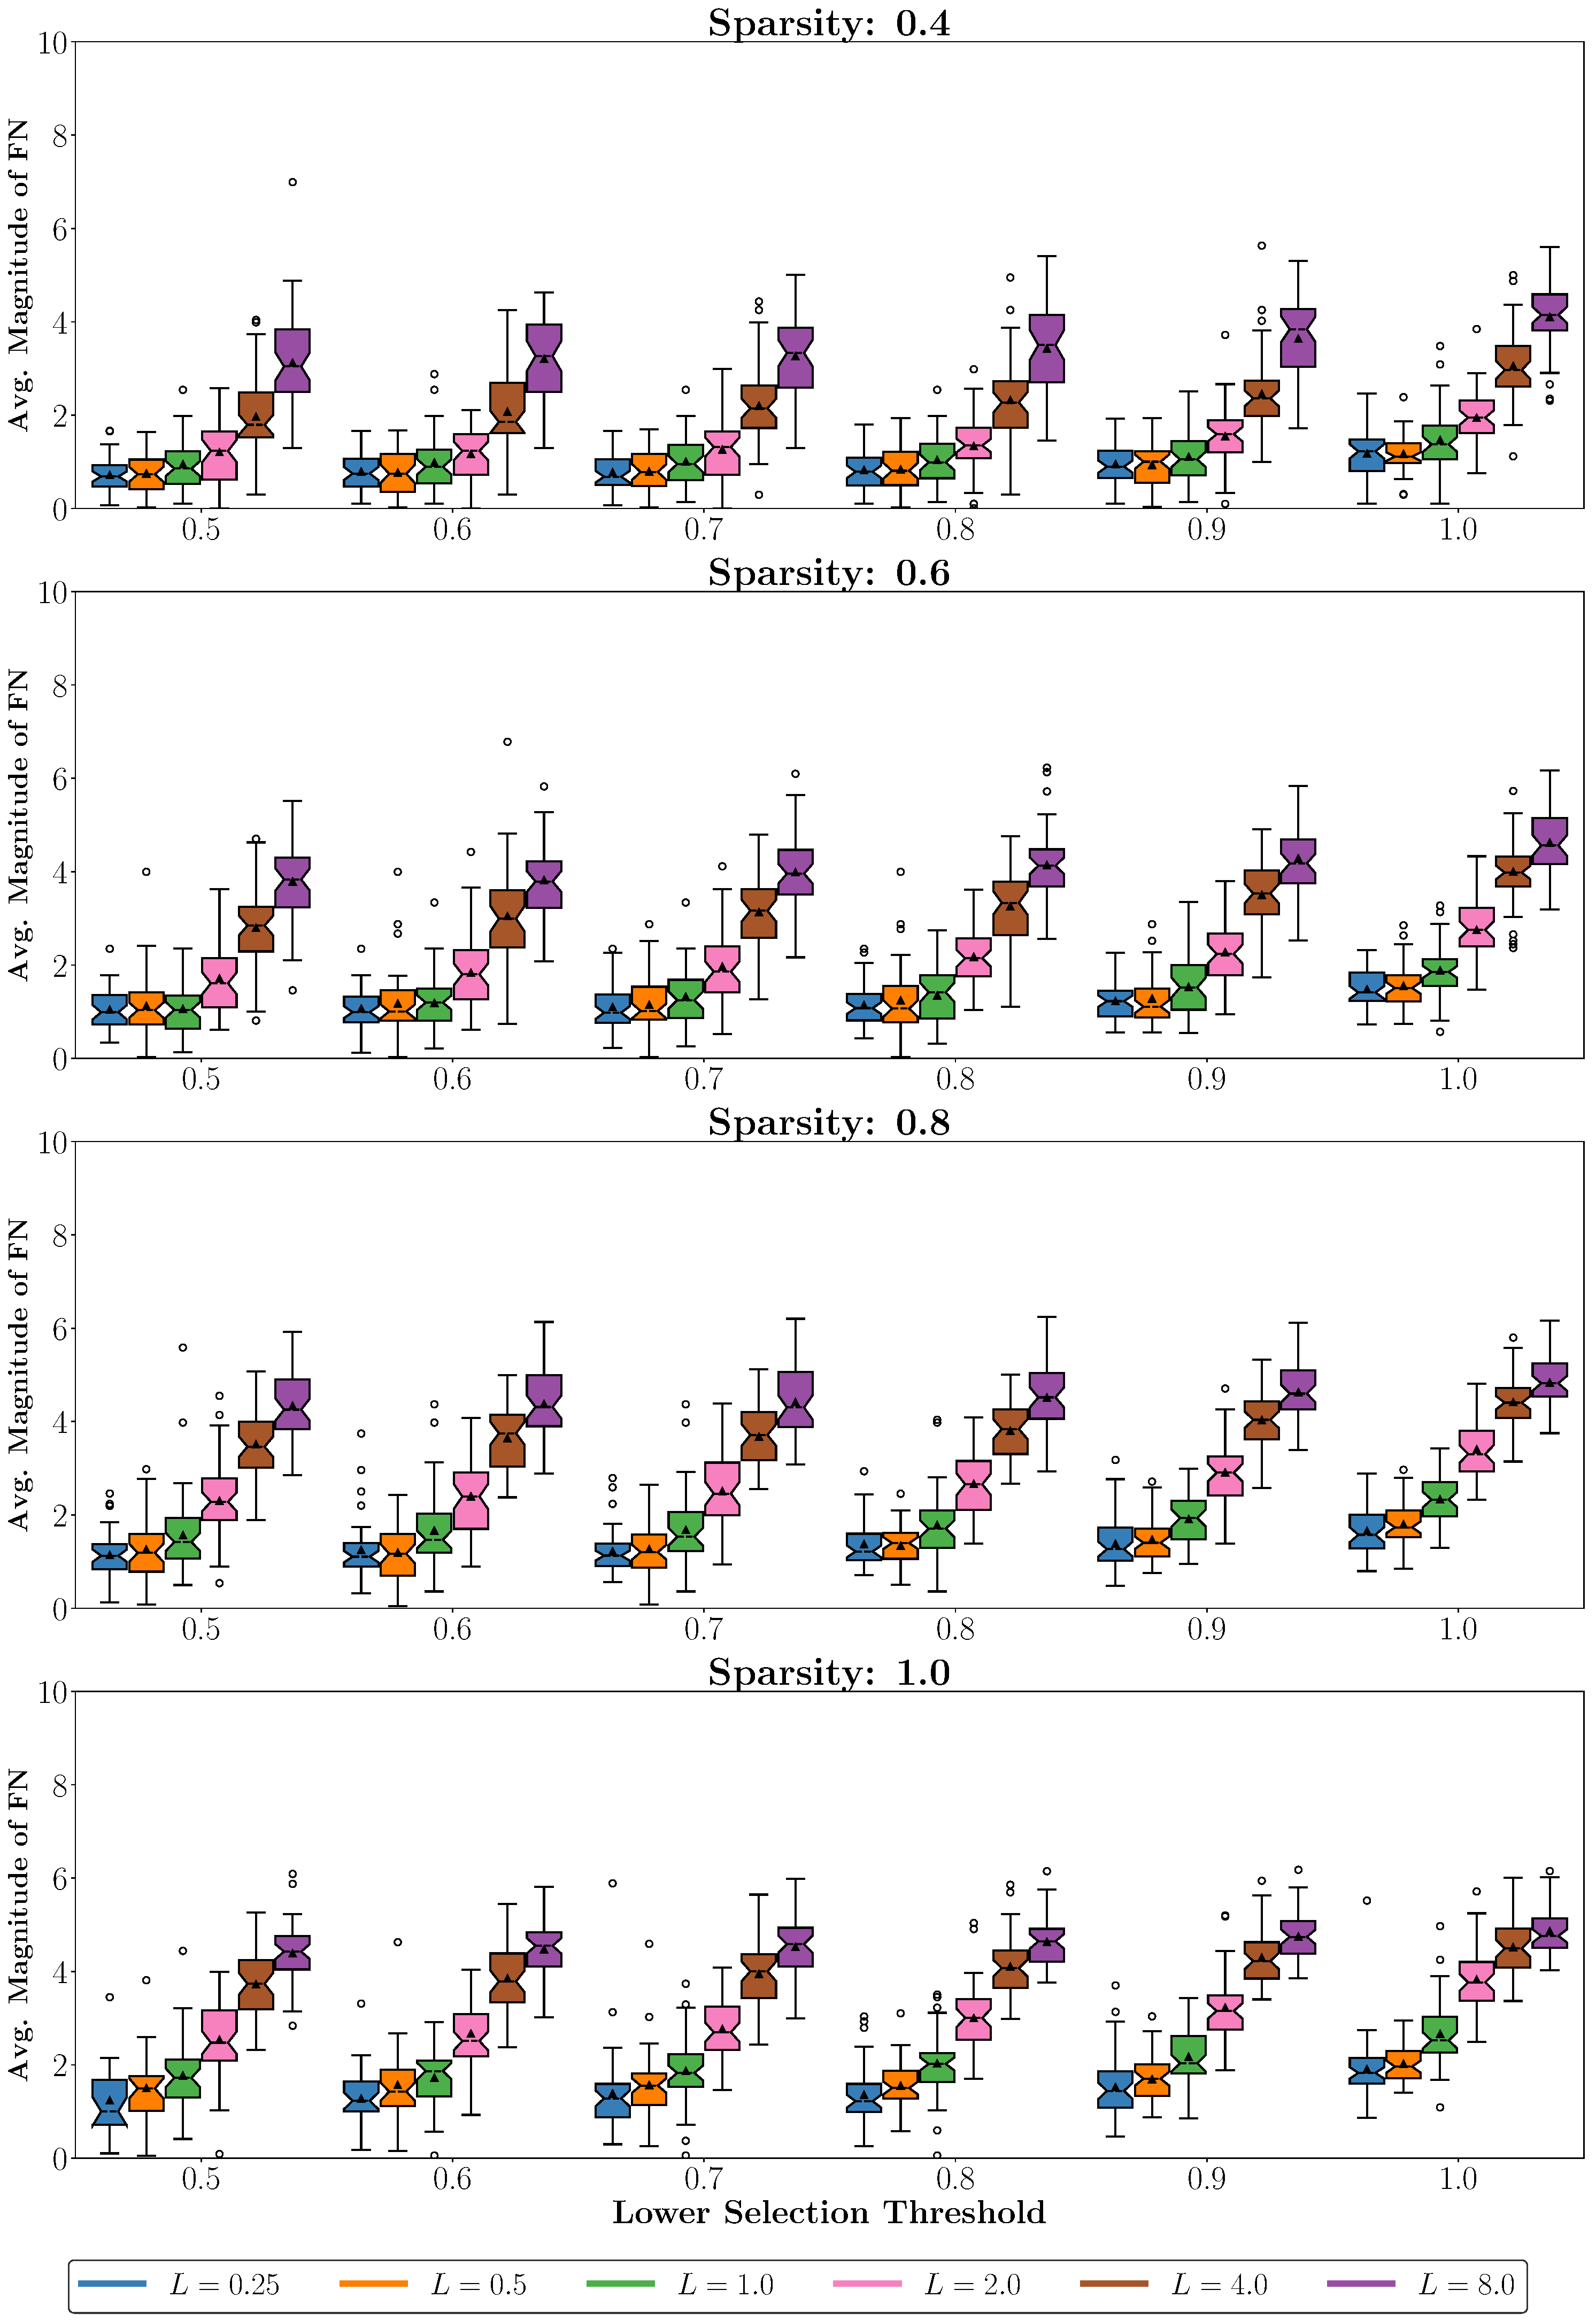
\includegraphics{img/exp3_mag_fn.pdf}}
	\caption{Average magnitude of false negatives. Boxplots are taken over datasets.}
	\label{fig:exp3-mag-fn}
\end{figure}

\begin{figure}[H]
	\centering
	\scalebox{0.25}{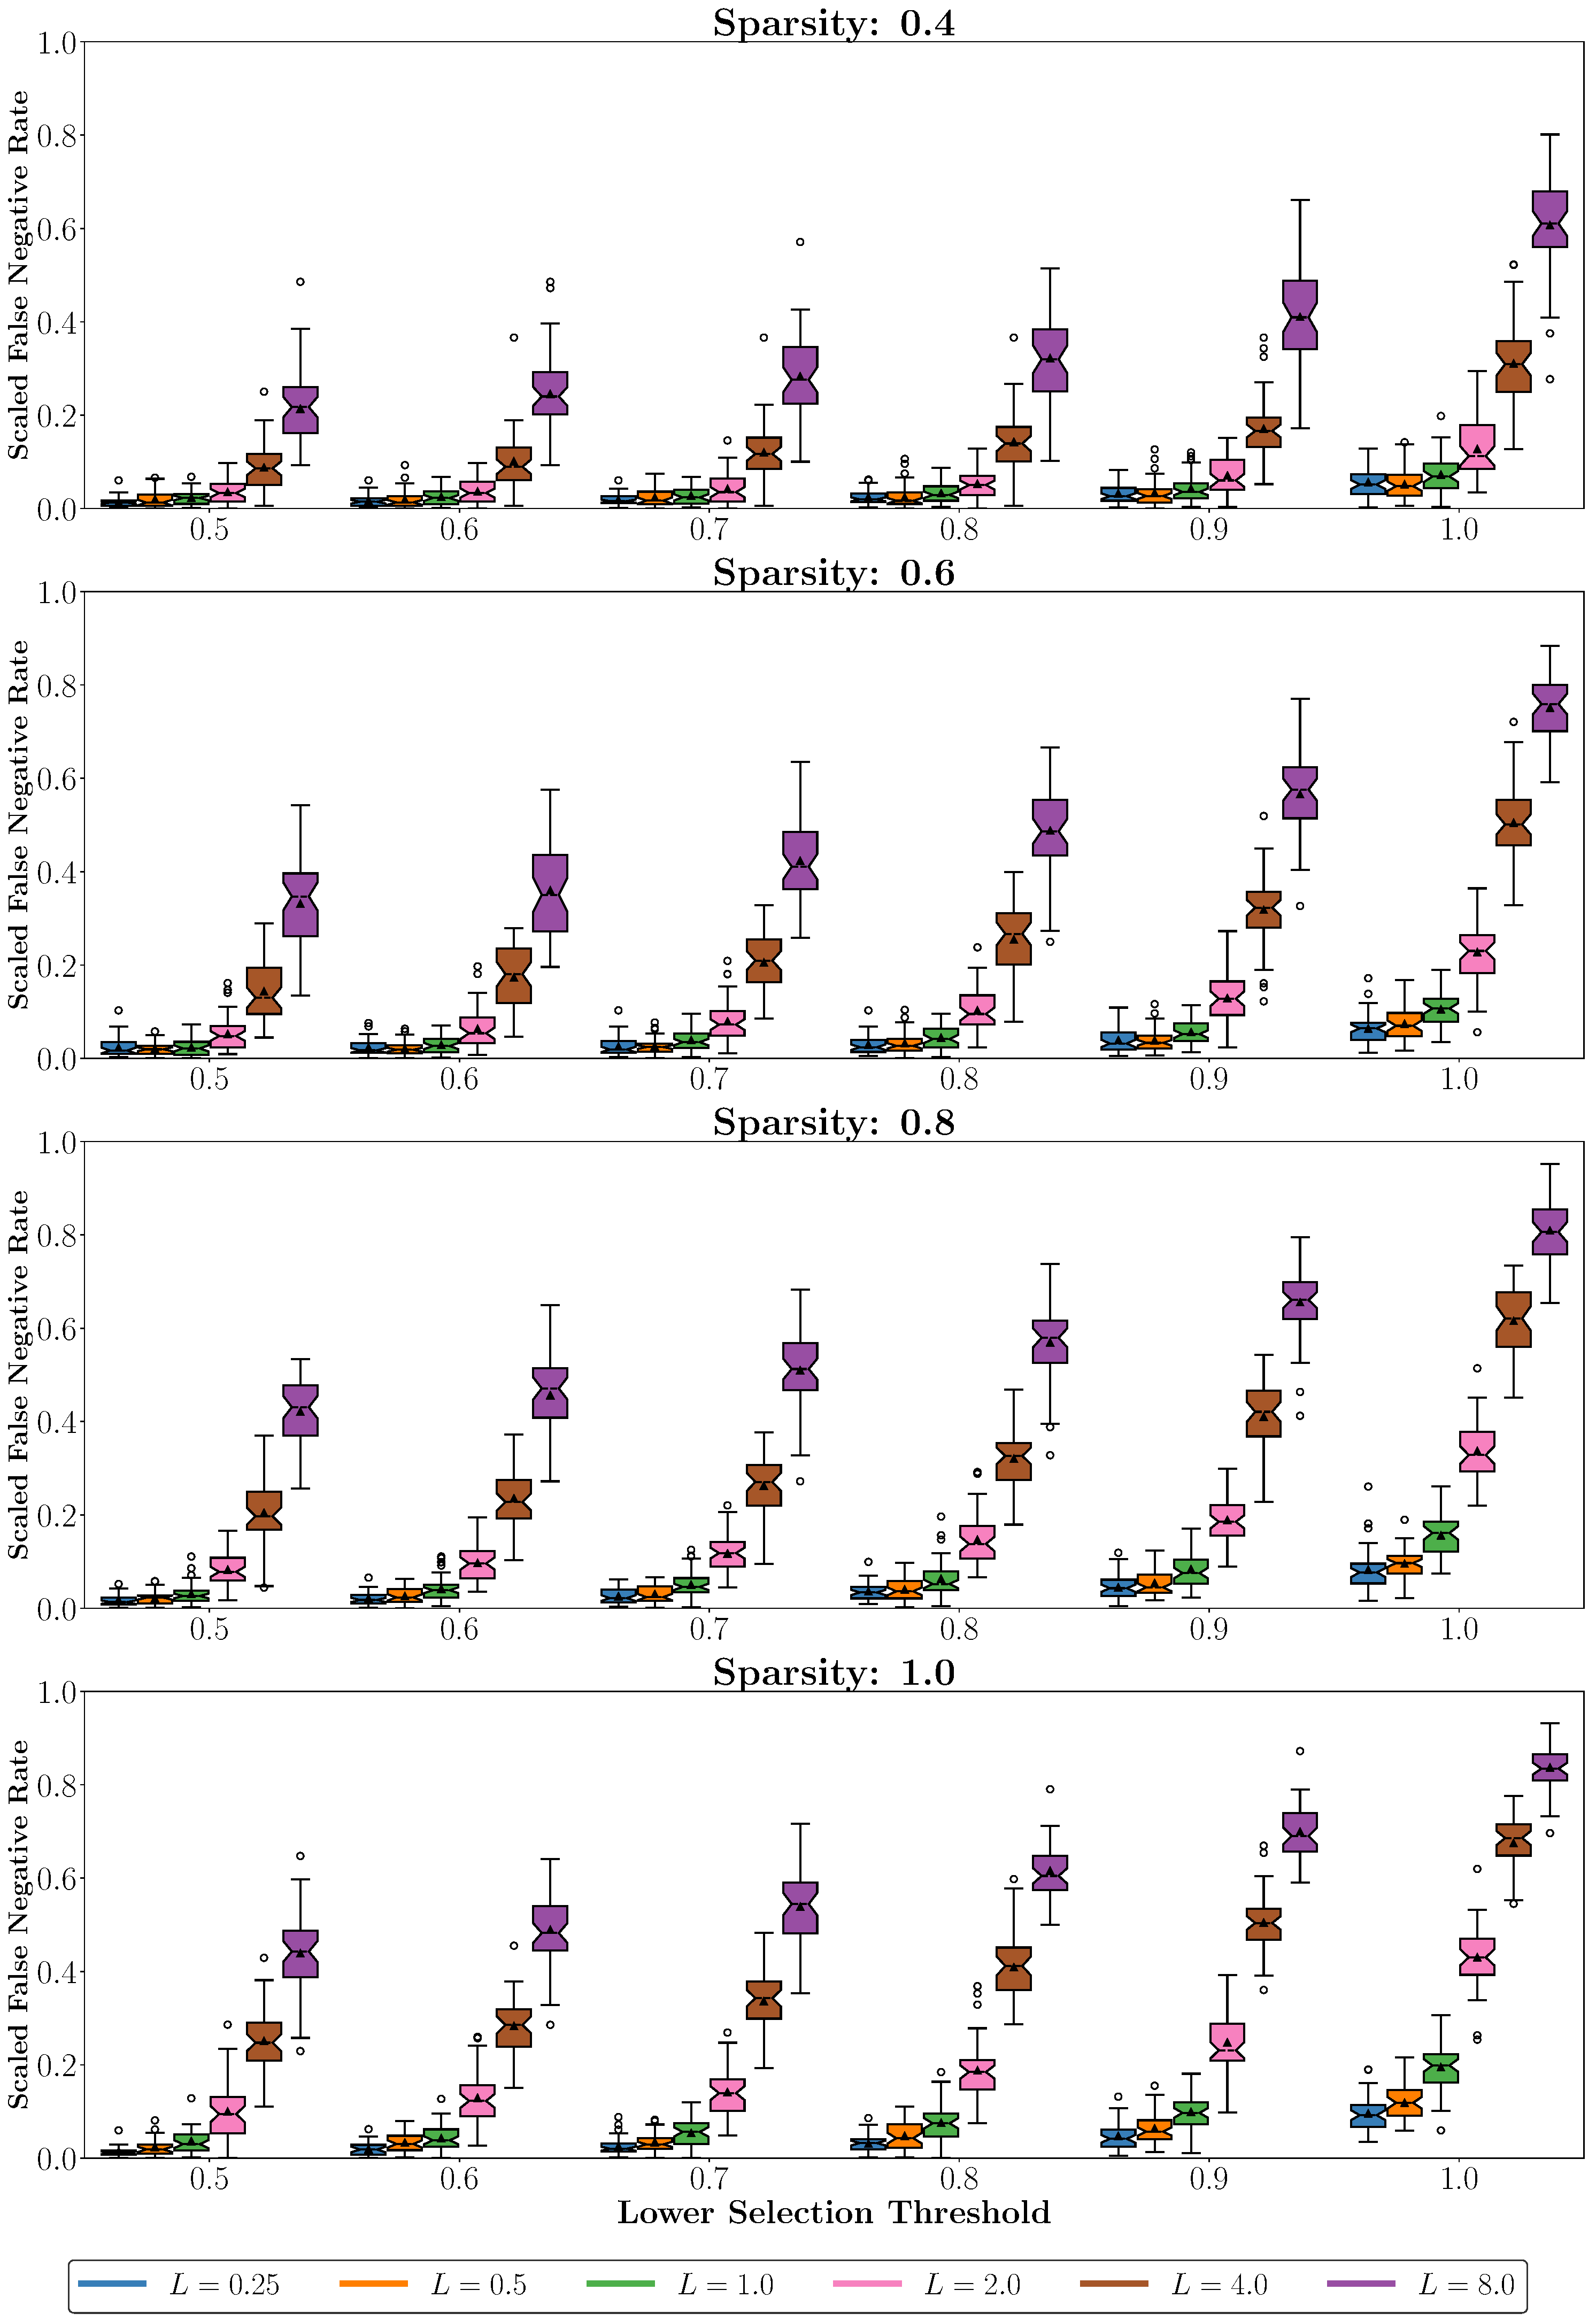
\includegraphics{img/exp3_mag_fn_scaled.pdf}}
	\caption{Scaled FNR. Boxplots are taken over datasets.}
	\label{fig:exp3-mag-fn-scaled}
\end{figure}

Next, we can examine the average magnitude of the false negatives across datasets as well as the scaled false negative rate (both defined explicitly in the previous section). These are shown in Figure \ref{fig:exp3-mag-fn} and Figure \ref{fig:exp3-mag-fn-scaled} above.  Lastly, we examine selection accuracy as a way to summarize the ROC results shown in Figure \ref{fig:exp3-sel-acc}. The selection accuracy highlights interesting behaviors. If the sparsity is very high, a decrease in LST will almost always improve selection accuracy. This increase is exaggerated if the correlations are stronger (larger $L$). If the sparsity is small, decreasing LST will harm selection accuracy performance since it will increase the number of false positives. This figure highlights, once again, that LST$=0.7$ is a good heuristic to follow.

\begin{figure}[H]
	\centering
	\scalebox{0.31}{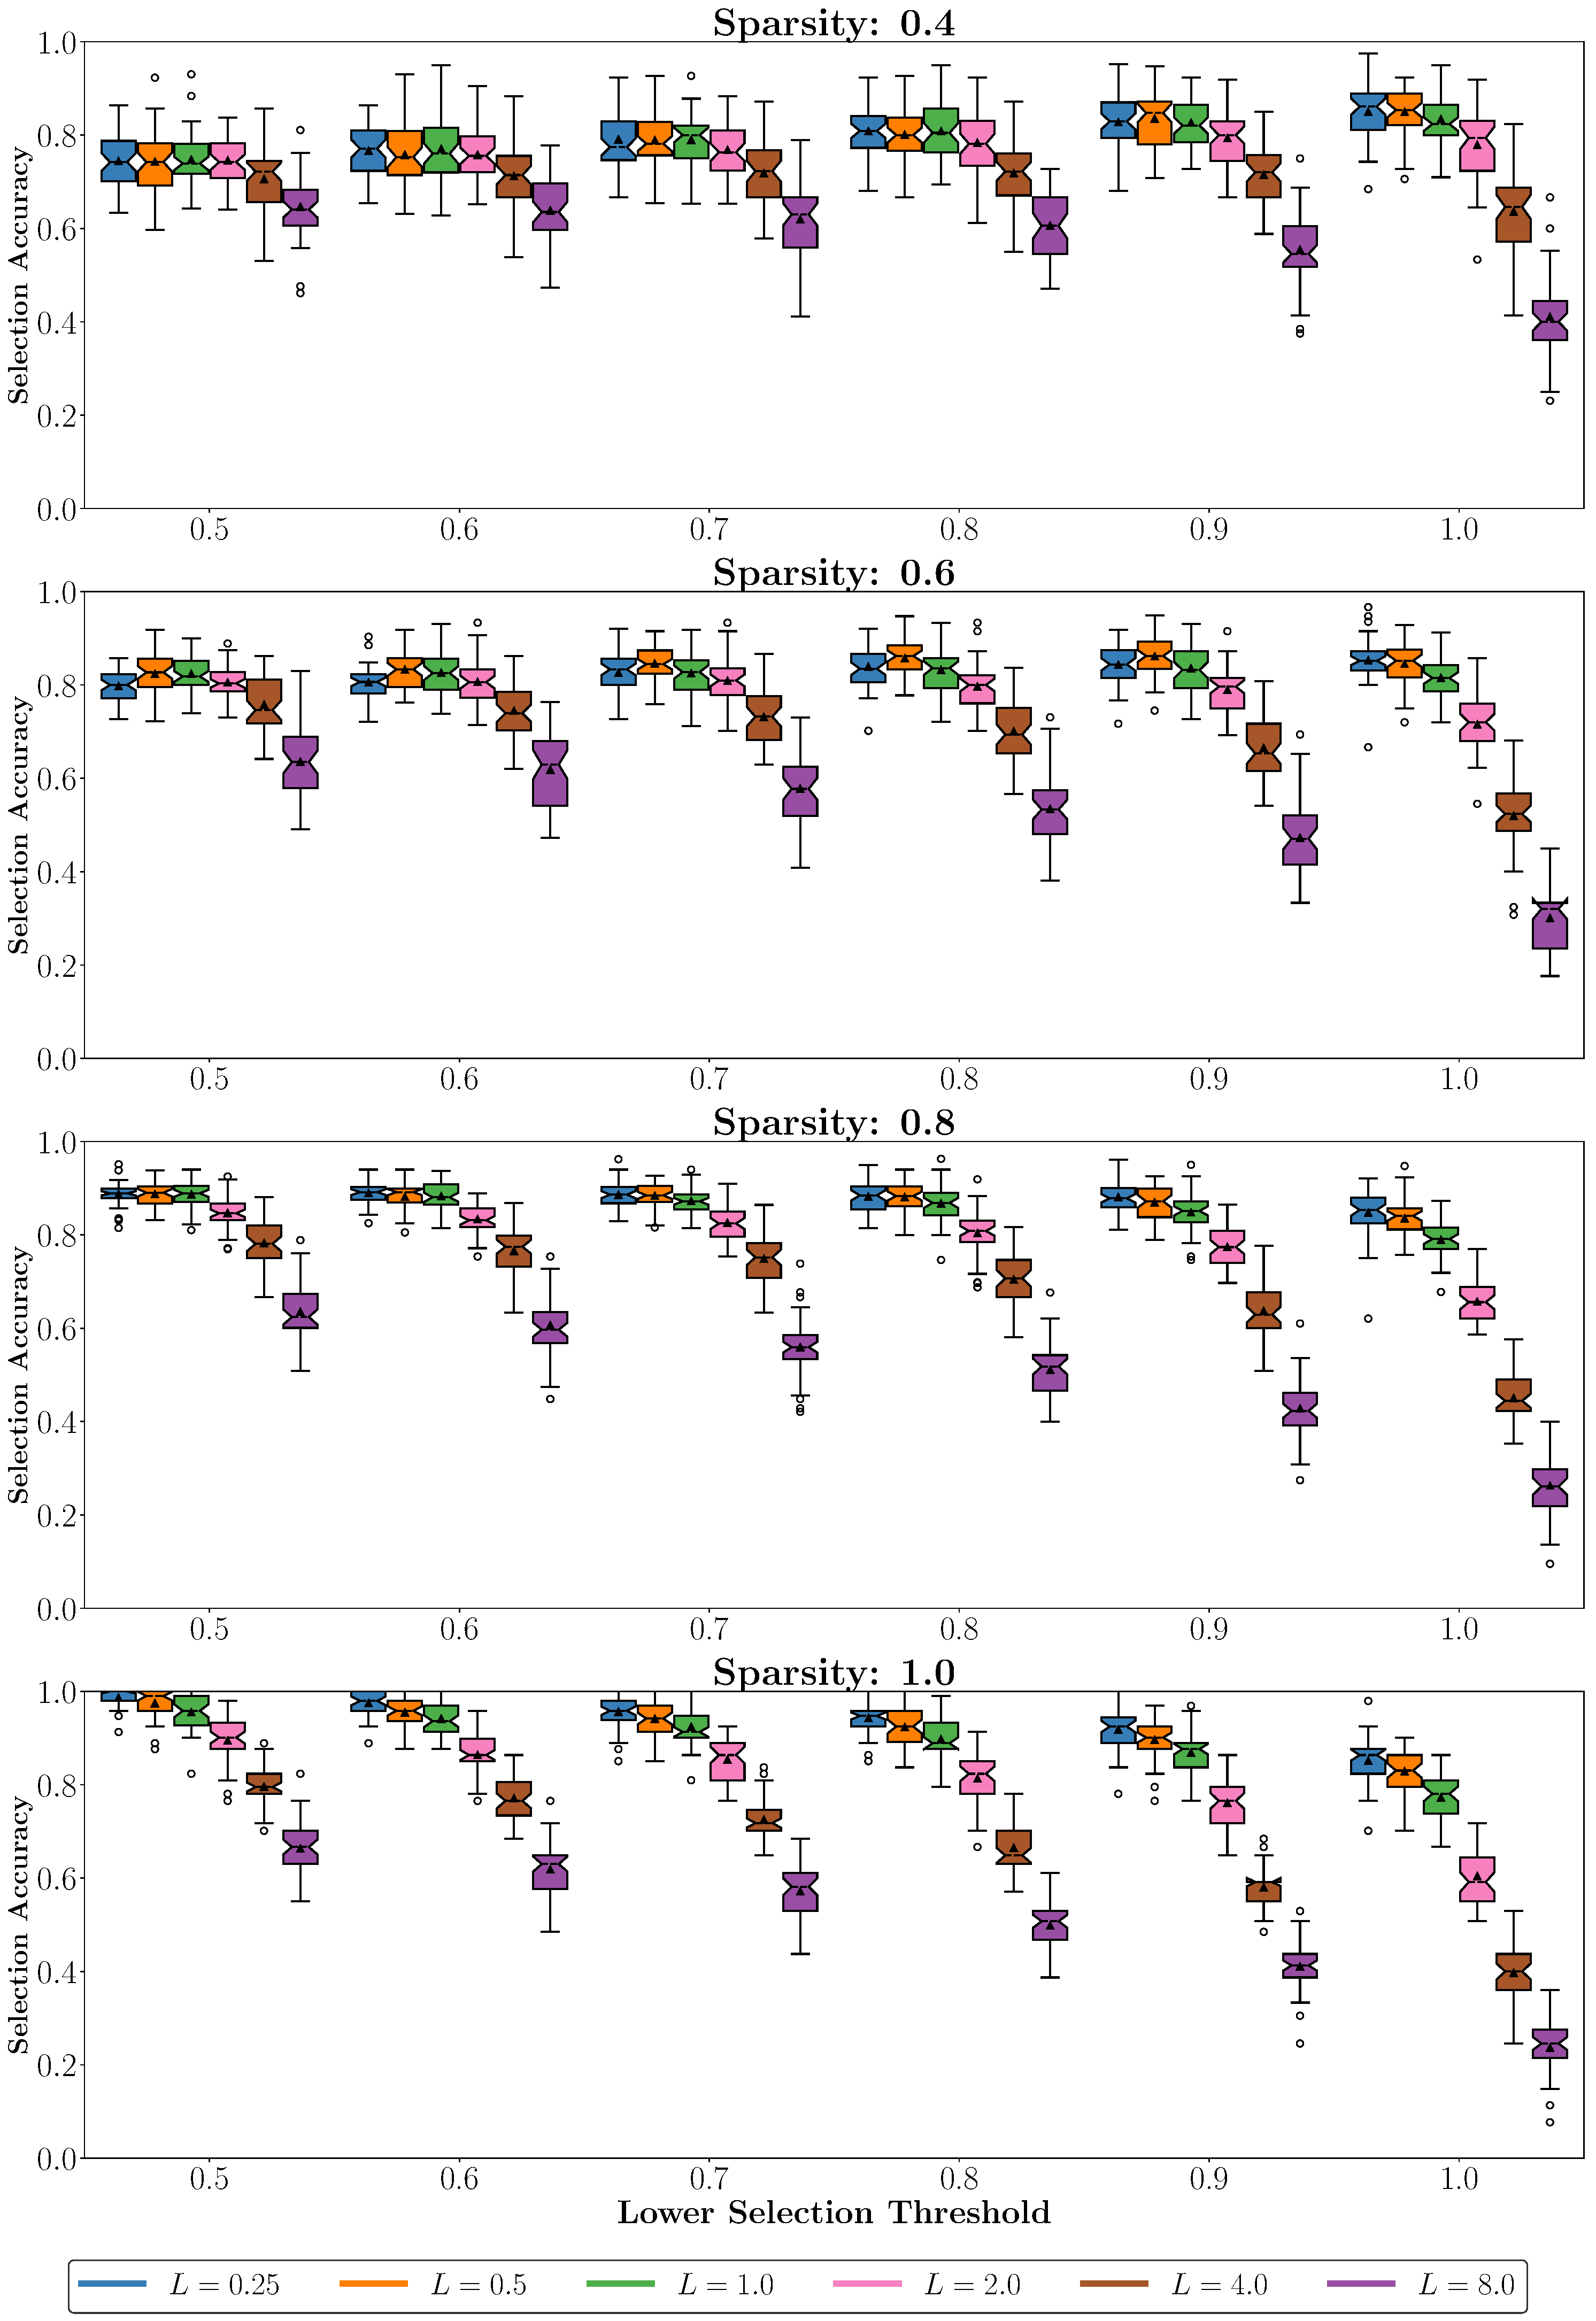
\includegraphics{img/exp3_sel_acc.pdf}}
	\caption{Average magnitude of false negatives. Boxplots are taken over datasets.}
	\label{fig:exp3-sel-acc}
\end{figure}
\end{document}
